\documentclass[12pt]{report}
\usepackage[utf8]{inputenc}
\usepackage{cite}
\usepackage[hidelinks]{hyperref}
\usepackage{graphicx}
\usepackage{amsfonts}
\usepackage{mathtools}
\usepackage{caption}
\usepackage{fancyhdr}
\usepackage[ruled,vlined]{algorithm2e}
\usepackage{float}

\pagestyle{fancy}
\fancyhf{}
\rhead{5-stage Pipelined Processor Report}
\lhead{\thesection}
\rfoot{\thepage}

\DeclarePairedDelimiter\ceil{\lceil}{\rceil}
\DeclarePairedDelimiter\floor{\lfloor}{\rfloor}

\title{\textbf{Computer Architecture} \\
\textbf{Final Assessment Report} \\
5-stage Pipelined Processor \\
Team \#4}
\author{
  Mohamed Shawky\\
  \small\texttt{SEC:2, BN:16}
  \and
  Remonda Talaat\\
  \small\texttt{SEC:1, BN:20}
  \and
  Evram Youssef\\
  \small\texttt{SEC:1, BN:9}
  \and
  Mahmoud Adas\\
  \small\texttt{SEC:2, BN:21}
}
\date{\today}

\begin{document}

\thispagestyle{empty}

\maketitle
\tableofcontents
\listoffigures
\listoftables
\clearpage

\pagenumbering{arabic}

\part{Introduction}
\section{Abstract}
This report describes our design work of the 5-stage pipelined processor, that follows Harvard architecture.

This report contains:
\begin{itemize}
    \item the overall system blocks and connections.
    \item the functionalities of the different blocks.
    \item the hazard solutions.
\end{itemize}

\part{Overall System Design}
\section{Overall System Design Schema}
Figure \ref{fig:overall} shows the overall system design in detail. Each unit is described in details in its section.
\begin{center}
    \begin{figure}[hp]
        \centering
        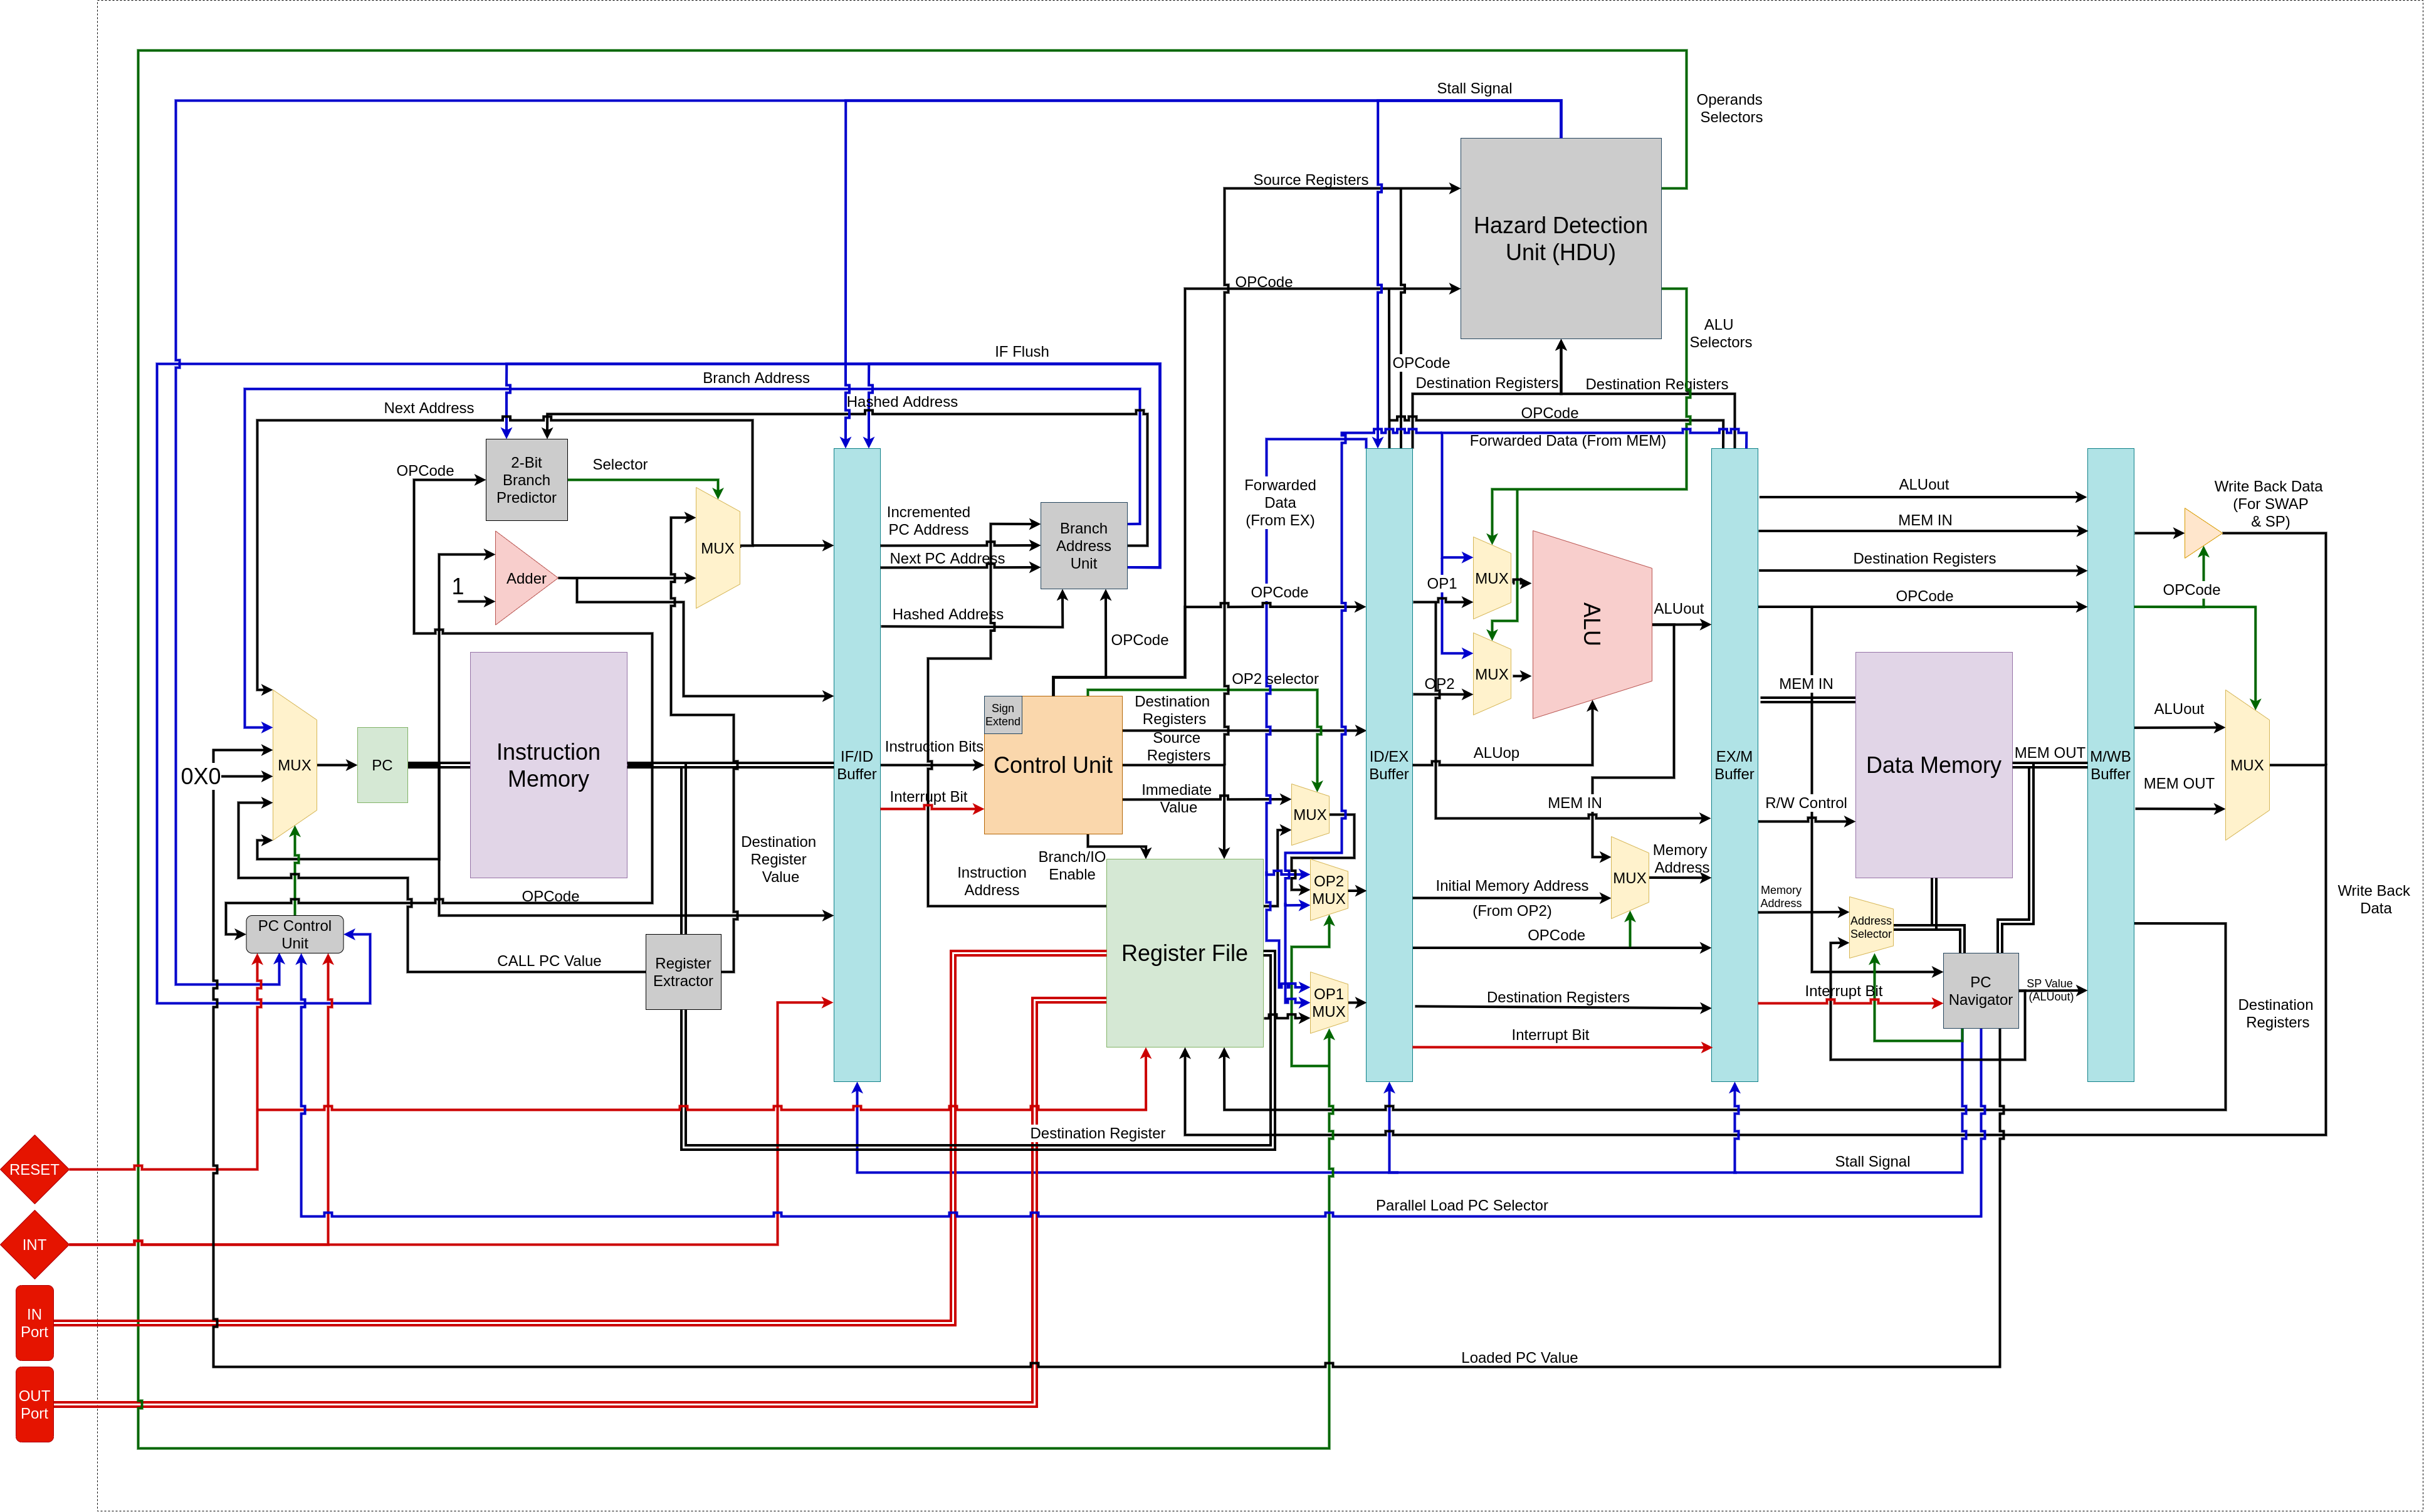
\includegraphics[width=\textwidth]{images/overall_system}
        \caption{Overall System Design}
        \label{fig:overall}
    \end{figure}
\end{center}

\section{Memory Specs}
The cpu follows Harvard architecture and thus uses the following 2 separate memory units:
\begin{itemize}
    \item Instructions Memory: Read-only, stores instructions.
    \begin{itemize}
        \item \textbf{Word Width}: 16 bits.
        \item \textbf{Address Bus Width}: 8 bits.
        \item \textbf{Data Bus Width}: 16 bits.
        \item \textbf{Total Number of Words}: $2^{16}$ words = 65,536 words = 131,072 bytes.
        \item \textbf{Valid Address Range}: From 0x0000 inclusive to 0xFFFF inclusive.
    \end{itemize}
    \item Data Memory: Read-Write, stores data and the stack.
    \begin{itemize}
        \item \textbf{Word Width}: 16 bits.
        \item \textbf{Address Bus Width}: 32 bits.\\
        \textit{For simulation}, this memory will ignore bits from (31 to 10) inclusive, and only work with bits from (9 to 0) inclusive.
        \item \textbf{Data Bus Width}: 32 bits.\\
        The higher bits (31 downto 16) are data at address A~.\\
        The lower bits (15 downto 0) are data at address A+1~.\\
        where $A ~mod~ 2 = 0$~.\\
        On read, data-memory loads data bus with data from A and A+1~.\\
        On write, data-memory stores data from data bus to both A and A+1 addresses.
        \item \textbf{Total Number of Words}: $2^{32}$ words = 4,294,967,296 words = 8,589,934,592 bytes.\\
        \textit{For simulation}, this memory will only have: $2^{10}$ words = 1,024 words = 2,048 bytes.
        \item \textbf{Valid Address Range}: Even Adresses From 0x0000\_0000 inclusive to 0xFFFF\_FFFF exclusive. Formaly $A \in $[0x0000\_0000, 0xFFFF\_FFFF) and $A ~mod~ 2 = 0$~.\\
        \textit{For simulation}, range will become: Even Addresses From 0x0000\_0000 inclusive to 0x0000\_0400 exclusive. Formaly $A \in $[0x0000\_0000, 0x0000\_0400) and $A ~mod~ 2 = 0$~.
    \end{itemize}
\end{itemize}

\section{PC Control Unit}

\subsection{Inputs}
\begin{itemize}
    \item IF Flush (1 bit)
    \item Stall Signal (1 bit)
    \item RESET Signal (1 bit)
    \item Interrupt Signal (1 bit)
    \item Current OPCode (7 bits)
    \item Parallel Load PC Selector (1 bit)
\end{itemize}

\subsection{Outputs}
\begin{itemize}
    \item PC Mux Selectors (3 bits)
\end{itemize}

\subsection{Logic}
\begin{itemize}
    \item If IF Flush == 1, Output = 001
    \item If RESET == 1, Output = 010
    \item If Stall == 1, Output = 011
    \item If Interrupt == 1 $||$ OPCode == RET/RTI, Output = 100
    \item PL PC Selector == 1, Output = 101
    \item Else, Output = 000
\end{itemize}

\section{Dynamic Branch Prediction}
Figure \ref{fig:bpu} shows the branch prediction unit.
\begin{center}
    \begin{figure}[hp]
        \centering
        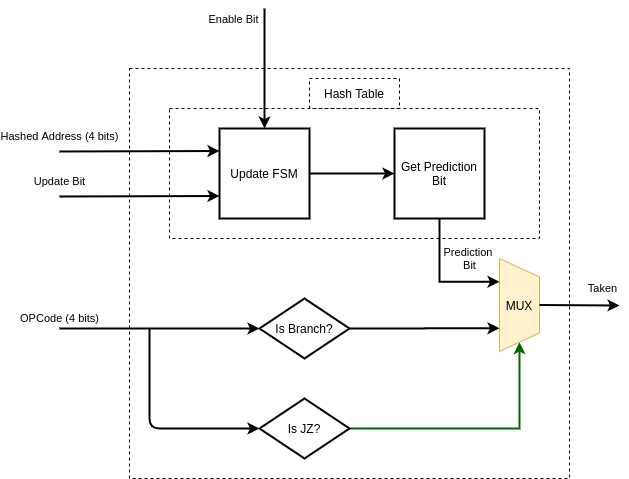
\includegraphics[width=0.8\textwidth]{images/bpu}
        \caption{Branch Prediction Unit Diagram}
        \label{fig:bpu}
    \end{figure}
\end{center}

\subsection{Inputs}
\begin{itemize}
    \item Hashed Address (4 bits)
    \item Update Bit (1 bit): \emph{Taken or Not}  to update FSM
    \item OPcode (4 bits)
\end{itemize}

\subsection{Outputs}
\begin{itemize}
    \item Taken (1 bit): predict whether the branch taken or not
\end{itemize}

\subsection{Logic}
\begin{itemize}
    \item Updates the FSM corresponding to the hashed address.
    \item Checks whether the OPCode is of a conditional branch instruction.
    \item Outputs the prediction bit \emph{(Taken or Not)} accordingly.
\end{itemize}

\section{Branch Address Unit}
Figure \ref{fig:bau} shows the branch address unit.
\begin{center}
    \begin{figure}[hp]
        \centering
        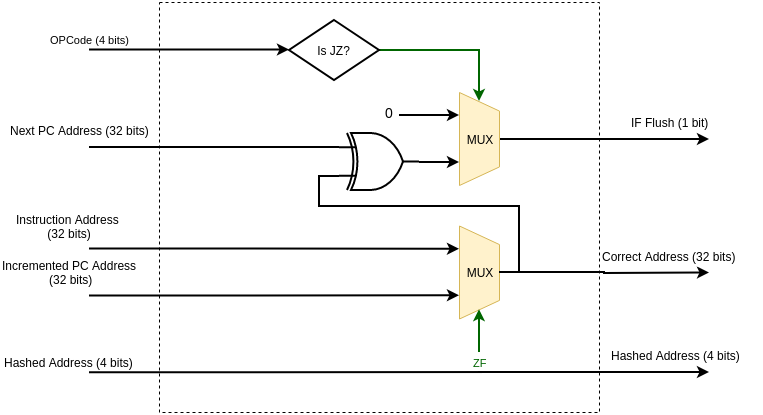
\includegraphics[width=0.8\textwidth]{images/bau}
        \caption{Branch Address Unit Diagram}
        \label{fig:bau}
    \end{figure}
\end{center}

\subsection{Inputs}
\begin{itemize}
    \item Next PC Address (32 bits)
    \item Instruction Address (32 bits)
    \item Incremented PC Address (32 bits)
    \item Hashed Address (4 bits)
    \item OpCode (4 bits)
\end{itemize}

\subsection{Outputs}
\begin{itemize}
    \item IF Flush (1 bit)
    \item Branch Address (32 bits)
    \item Hashed Address (4 bits)
    % TODO: why is Hashed address repeated?
\end{itemize}

\subsection{Logic}
\begin{itemize}
    \item Check if OpCode is of a conditional branch instruction, if true:
    \begin{itemize}
        \item Check whether PC Next Address is equal to Instruction Address
        \item If true:
        \begin{itemize}
            \item IF Flush = 0, Branch Address = Instruction Address
        \end{itemize}
        \item If false:
        \begin{itemize}
            \item IF Flush = 1, Branch Address = Instruction Address
        \end{itemize}
    \end{itemize}
    % TODO: what heppens if OpCode is not branch?
\end{itemize}

\section{Register File}
Figure \ref{fig:reg_file} shows the register file.

\subsection{Registers}
\begin{itemize}
    \item 8 general purpose registers each of size 32 bits
    \item Stack pointer (SP) register (32 bits)
    \item Program counter (PC) register (32 bits)
\end{itemize}

\subsection{Inputs}
\begin{itemize}
    % TODO: what is the mapping of the selectors?
    \item Dest Regs: 2$\times$4 bits (for destination selection)
    \item SRC Regs: 2$\times$4 bits (for source selection)
    % TODO: what is the address for PC and SP?
    \item Fetch Reg: 4 bits (for fetch branch register selection)
    \item WB values: 2$\times$32 bits (for write back values)
    \item RESET: 1 bit (for registers clear).
    \item Branch/IO: 2 bits (to determine whether the operation is IO or branch)
    \item IN Port: 32 bits (IO input port)
\end{itemize}

\subsection{Outputs}
\begin{itemize}
    \item OP1: 32 bits (value of first operand)
    \item OP2: 32 bits (value of second operand)
    \item Fetch Value: 32 bits (value of branch address required by fetch)
    \item Instruction Address: 32 bits (value of branch address)
    \item OUT Port: 32 bits (IO output port)
\end{itemize}

\subsection{Logic}
The register selector acts like a decoder to select the required operation and the register on which the operation performed.

\begin{center}
    \begin{figure}[hp]
        \centering
        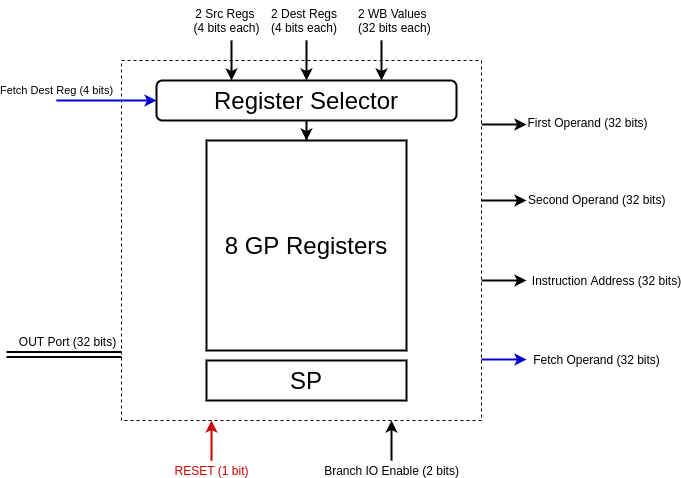
\includegraphics[width=0.8\textwidth]{images/reg_file}
        \caption{Register File Diagram}
        \label{fig:reg_file}
    \end{figure}
\end{center}

\section{ALU}

\subsection{Inputs}
\begin{itemize}
    \item ALUop: 4 bits (refer to ALU Operations below)
    \item Operands: 2$\times$32 bits (2 input operands)
\end{itemize}

\subsection{Outputs}
\begin{itemize}
    \item ALUout: 32 bits (operation result)
\end{itemize}

\subsection{ALU Operations}
\begin{itemize}
    \item 0000 $-$ NOP $-$ (no operation)
    \item 0001 $-$ INC $-$ (first operand + 1)
    \item 0010 $-$ DEC $-$ (first operand - 1)
    \item 0011 $-$ ADD $-$ (first operand + second operand)
    \item 0100 $-$ SUB $-$ (first operand - second operand)
    \item 0101 $-$ AND $-$ (first operand \&\& second operand)
    \item 0110 $-$ OR $-$ (first operand $||$ second operand)
    \item 0111 $-$ NOT $-$ (!first operand)
    \item 1000 $-$ SHL $-$ (shift first operand to the left with the value of second operand)
    \item 1001 $-$ SHR $-$ (shift first operand to the right with the value of second operand)
    \item 1010 $-$ INC2 $-$ (first operand + 2)
    \item 1011 $-$ DEC2 $-$ (first operand - 2)
\end{itemize}

\subsection{Logic}
\begin{itemize}
    \item ALU performs the operation and changes the CCR accordingly.
    \item The input operands of the ALU are multiplexed between forwarded data and register data, with selectors from data forwarding unit.
\end{itemize}


\section{PC Navigator}
Figure \ref{fig:pc_nav} shows the PC Navigator.

\begin{figure}[hp]
    \centering
    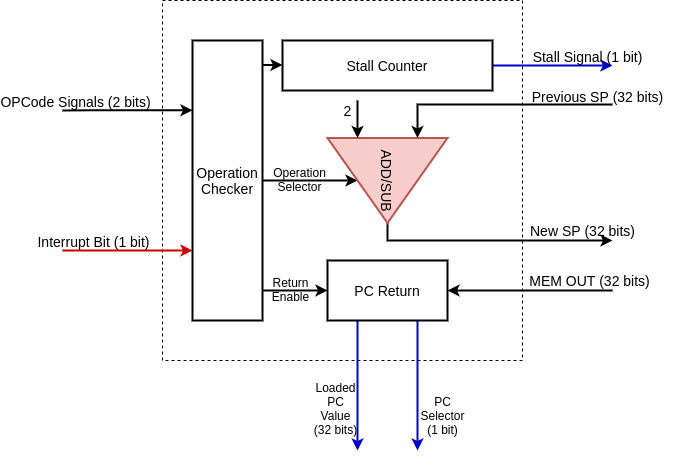
\includegraphics[width=0.8\textwidth]{images/pc_nav.png}
    \caption{PC Navigator Diagram}
    \label{fig:pc_nav}
\end{figure}

\subsection{Inputs}
\begin{itemize}
    \item Interrupt Bit (1 bit)
    \item OPCode Signals (2 bits): to check whether the operation is RET or RTI
    \item Previous SP (32 bits): to increment or decrement it correspondingly to access Data Memory
    \item MEM OUT (32 bits): loaded PC from memory
\end{itemize}

\subsection{Outputs}
\begin{itemize}
    \item Stall Signal (1 bit)
    \item New SP (32 bits)
    \item PC Selector (1 bit): to enable PC parallel load from Data Memory
    \item Loaded PC Value (32 bits)
\end{itemize}

\subsection{Logic}
\begin{itemize}
    \item The Operation Checker checks the OPCode Signals and Interrupt Bit to check whether the operation is RET, RTI or Interrupt and produces its signals accordingly:
    \begin{itemize}
        \item PC Return Enable is set.
        \item Counter is set to $0$ for RET, $1$ for RTI and $2$ for Interrupt.
        \item Operation Selector is issued to the Adder/Subtractor to change the value of SP.
    \end{itemize}
    \item Stall Counter counts the number of stalls produced by operation. It's set to $0$ for RET, $1$ for RTI and $2$ for Interrupt. It counts down a number of cycles and then release the stall.
    \item Adder/Subtractor is used to update the SP every stall cycle, to get the right data from the memory.
    \item PC Return issues a signal to the PC Control Unit to enable parallel load from data memory and passes the loaded PC value.
    \item RET doesn't stall any cycles, as it only loads PC value from data memory.
    \item RTI stall only one cycle, as it loads PC value from data memory and then loads CCR.
    \item Interrupt stall two cycles, as it loads PC value from data memory, pushes CCR into stack and then pushes PC into stack.
\end{itemize}


\part{Instruction Format}
\section{One Operand Operations}
\begin{itemize}
    \item 4 bits (1111) for one operand instructions.
    \item 3 bits to define instruction.
    \item 3 bits for destination register.
    \item 1 bit to define the memory slots occupied by the instruction.
    \item Total of 11 bits, padded with 5 0's to fit 16 bits.
\end{itemize}
\begin{center}
    \captionof{table}{One Operand Instruction Mapping\label{tab:1op}}
 \begin{tabular}{||c| c| c| c| p{40mm}||} 
 \hline
 Operation & OpCode & Destination & 16$|$32 & Conditions  \\ [0.5ex] 
 \hline\hline
 IN & 1111000 & 000:111 & 0 & ----------------------- \\
 \hline
 NOT & 1111001 & 000:111 & 0 & if !Rdst=0,Z=1 \newline if !Rdst$<$0,N=1 \\
 \hline
 INC & 1111010 & 000:111 & 0 & if Rdst+1=0,Z=1 \newline if Rdst+1$<$0,N=1 \\
 \hline
 DEC & 1111011 & 000:111 & 0 & if Rdst-1=0,Z=1 \newline if Rdst-1$<$0,N=1 \\
 \hline
 OUT & 1111100 & 000:111 & 0 & ----------------------- \\
 \hline
\end{tabular}
\end{center}

\section{Special Operations}
\begin{itemize}
    \item 16 0's to represent NOP (0000000000000000).
\end{itemize}

\section{Two Operand Operations}
\begin{itemize}
    \item 4 bits to define instruction.
    \item 3 bits for each of Rsrc1, Rsrc2 and Rdst.
    \item 1 bit to define the memory slots occupied by the instruction.
    \item 16 bits for immediate values.
    \item Total of 14 bits in most cases with some exceptions mentioned below.
\end{itemize}
\begin{center}
    \captionof{table}{Two Operand Instruction Mapping\label{tab:1op}}
 \begin{tabular}{||c| c| c| c| c| c| c| p{30mm}||} 
 \hline
 Operation & OpCode & Rsrc1 & Rsrc2 & Rdst & imm & 16$|$32 & Conditions  \\ [0.5ex] 
 \hline\hline
 SWAP & 0001 & 000:111 & --- & 000:111 & --- & 0 & ----------------------- \\
 \hline
 ADD & 0010 & 000:111 & 000:111 & 000:111 & --- & 0 & if Result=0,Z=1 \newline if Result$<$0,N=1 \\
 \hline
 SUB & 0011 & 000:111 & 000:111 & 000:111 & --- & 0 & if Result=0,Z=1 \newline if Result$<$0,N=1 \\
 \hline
 AND & 0100 & 000:111 & 000:111 & 000:111 & --- & 0 & if Result=0,Z=1 \newline if Result$<$0,N=1 \\
 \hline
 OR & 0101 & 000:111 & 000:111 & 000:111 & --- & 0 & if Result=0,Z=1 \newline if Result$<$0,N=1 \\
 \hline
 SHL & 0110 & 000:111 & --- & --- & 16 bits & 1 & update carry flag \\
 \hline
 SHR & 0111 & 000:111 & --- & --- & 16 bits & 1 & update carry flag \\
 \hline
 IADD & 1000 & 000:111 & --- & 000:111 & 16 bits & 1 & if Result=0,Z=1 \newline if Result$<$0,N=1 \\
 \hline
\end{tabular}
\end{center}

\section{Memory Operations}
\begin{itemize}
    \item 4 bits to define instruction.
    \item 3 bits for destination register.
    \item 1 bit to define the memory slots occupied by the instruction.
    \item 16 bits for immediate values.
    \item 20 bits for effective addresses.
    \item Total of 8 bits with no immediate values or effective addresses.
    \item Total of 24 bits with immediate values.
    \item Total of 28 bits with effective addresses.
\end{itemize}
\begin{center}
    \captionof{table}{Memory Instruction Mapping\label{tab:1op}}
 \begin{tabular}{||c| c| c| c| c| c| p{40mm}||} 
 \hline
 Operation & OpCode & Rdst & imm & EA & 16$|$32 & Conditions  \\ [0.5ex] 
 \hline\hline
 PUSH & 1001 & 000:111 & --- & --- & 0 & ----------------------- \\
 \hline
 POP & 1010 & 000:111 & --- & --- & 0 & ----------------------- \\
 \hline
 LDM & 1011 & 000:111 & 16 bits & --- & 1 & ----------------------- \\
 \hline
 LDD & 1100 & 000:111 & --- & 20 bits & 1 & ----------------------- \\
 \hline
 STD & 1101 & 000:111 & --- & 20 bits & 1 & ----------------------- \\
 \hline
\end{tabular}
\end{center}

\section{Branch and Change Control Operations}
\begin{itemize}
    \item 4 bits (0000) for branching instructions.
    \item 3 bits to define instruction.
    \item 3 bits for destination register.
    \item 1 bit to define the memory slots occupied by the instruction.
    \item Total of 11 bits, padded with 5 0's to fit 16 bits. 
\end{itemize}
\begin{center}
    \captionof{table}{One Operand Instruction Mapping\label{tab:1op}}
 \begin{tabular}{||c| c| c| c| p{40mm}||} 
 \hline
 Operation & OpCode & Destination & 16$|$32 & Conditions  \\ [0.5ex] 
 \hline\hline
 JZ & 0000001 & 000:111 & 0 & ----------------------- \\
 \hline
 JMP & 0000010 & 000:111 & 0 & ----------------------- \\
 \hline
 CALL & 0000011 & 000:111 & 0 & ----------------------- \\
 \hline
 RET & 0000100 & --- & 0 & ----------------------- \\
 \hline
 RTI & 0000101 & --- & 0 & ----------------------- \\
 \hline
\end{tabular}
\end{center}

\part{Control Unit (Signals)}

\section{Overview}
Control unit is responsible for generating the control signals that are used to activate several operations throughout the pipeline. Also, it's responsible for the extraction of specific information from instruction bits.

\begin{itemize}
    \item It communicates with:
    \begin{itemize}
        \item IF/ID buffer: for reading the instruction bits.
        \item ID/EX buffer: for writing the appropriate registers, ALUop and signals.
        \item Register file: for selecting the registers needed to be read (Rsrc1 and Rsrc2).
        \item Hazards units (HDU and Branch Address Unit): for sending enables and needed signals.
    \end{itemize}
    
    \item Unit Interface:
    \begin{itemize}
    
        \item Inputs: 
        \begin{itemize}
            \item Instruction Bits (32 bits)
            \item Interrupt bit (1 bit)
        \end{itemize}
        
        \item Outputs:
        \begin{itemize}
            \item Rsrc2\_val (32 bits) for immediate values or effective addresses
            \item Rsrc1\_sel (4 bits)
            \item Rsrc2\_sel (4 bits)
            \item Rdst1\_sel (4 bits)
            \item Rdst2\_sel (4 bits) used only in case of swap
            \item Branch/IO Enable (2 bits)
            \item OP2\_sel (1 bit)
            \item SP Enable (1 bit)
            \item OpCode (7 bits)
            \item Branch Enable (1 bit)
            \item ALUop (4 bits)
            \item R/W Control Signal (2 bits)
        \end{itemize}
        
    \end{itemize}
    
    \item Interpretation:
    \begin{itemize}
        \item \textbf{Rsrc2\_val (32 bits):} occupies a single place in the ID/EX buffer. However, it's used in many different ways. It can be used as a register value extracted form register file. it can be used as an immediate value extracted from IF/ID buffer. Also, it can hold the stack pointer address, as well as the effective address (EA) sent to the memory for reading or writing.
        \item \textbf{Rdst2 (4 bits):} only used when dealing with a SWAP instruction, thus we need Op1 and Op2 and their new selectors.
        \item \textbf{OP2\_sel (1 bit):} determines the value of Rsrc2 register in ID/EX buffer, whether it's immediate or register value.
        \item  \textbf{Branch/IO Enable (2 bits):} informs the register file what operation of these are we executing (No/In/Out/Branch), however \emph{Branch Enable} (1 bit) interacts with the Branch Address Unit, informing it what type of OpCode are we dealing with (branching or not).
    \end{itemize}
\end{itemize}

\section{Control Signals}
In this section, instructions are divided into seven types based on the signals produced:
\begin{itemize}
    \item One Operand (not,inc,dec,out,in).
    \item Two Operands (add,sub,and,or).
    \item Immediate Operand (iadd,shl,shr,ldm).
    \item Data (ldd,std).
    \item Stack (push,pop,call,ret,rti).
    \item Jump (jz, jmp).
    \item Special (nop,swap,reset,int).
\end{itemize}   

\subsection{One Operand Instructions}
\begin{itemize}
    \item IB[31:0] are the instruction bits.
    \item Inserting (1111) to Rsrc/Rdst selectors informs the register file not to output any register values.
    \item 'x' indicates don't care.
    \item 0000 at the ALUop indicates no operation.
    \item Rsrc1\_sel is the same as Rdst1\_sel.
\end{itemize}

\begin{center}
    \captionof{table}{One Operand Instruction Control Signals Part I\label{tab:1op1}}
\begin{tabular}{||p{20mm}| p{15mm}| p{15mm}| p{15mm}| p{15mm}| p{15mm}| p{15mm}||} 
\hline
Instruction & OPCode & ALUop & Rsrc1 selector & Rsrc2 selector & Rdst1 selector & Rsrc2 value \\ [0.5ex] 
\hline\hline
NOT & IB[31:25] & 0111 & 0 and IB[24:22] & 1111 & 0 and IB[24:22] & x  \\
\hline
INC & IB[31:25] & 0001 & 0 and IB[24:22] & 1111 & 0 and IB[24:22] & x \\
\hline
DEC & IB[31:25] & 0010 & 0 and IB[24:22] & 1111 & 0 and IB[24:22] & x \\
\hline
OUT & IB[31:25] & 0000 & 0 and IB[24:22] & 1111 & 0 and IB[24:22] & x \\
\hline
IN  & IB[31:25] & 0000 & 0 and IB[24:22] & 1111 & 0 and IB[24:22] & x \\
\hline
\end{tabular}
\end{center}

\begin{center}
    \captionof{table}{One Operand Instruction Control Signals Part II\label{tab:1op2}}
\begin{tabular}{||p{20mm}| p{15mm}| p{15mm}| p{15mm}| p{15mm}| p{15mm}| p{15mm}||} 
\hline
Instruction & OP2 selector & Rdst2 (swap) & Branch /IO Enable & SP Enable & Branch Enable & R/W Control Signal \\ [0.5ex] 
\hline\hline
NOT & x & 1111 & 00 & 0 & 0 & 00 \\
\hline
INC & x & 1111 & 00 & 0 & 0 & 00 \\
\hline
DEC & x & 1111 & 00 & 0 & 0 & 00 \\
\hline
OUT & x & 1111 & 01 & 0 & 0 & 00 \\
\hline
IN  & x & 1111 & 10 & 0 & 0 & 00 \\
\hline
\end{tabular}
\end{center}

\subsection{Two Operand Instructions}
\begin{itemize}
    \item OP2\_sel: 0 the register value and 1 the imm/ea value.
\end{itemize}

\begin{center}
    \captionof{table}{Two Operands Instruction Control Signals Part I\label{tab:2op1}}
\begin{tabular}{||p{20mm}| p{15mm}| p{15mm}| p{15mm}| p{15mm}| p{15mm}| p{15mm}||} 
\hline
Instruction & OPCode & ALUop & Rsrc1 selector & Rsrc2 selector & Rdst1 selector & Rsrc2 value  \\ [0.5ex] 
\hline\hline
ADD & IB[31:25] & 0011 & 0 and IB[27:25] & 0 and IB[24:22] & 0 and IB[21:19] & x \\
\hline
SUB & IB[31:25] & 0100 & 0 and IB[27:25] & 0 and IB[24:22] & 0 and IB[21:19] & x \\
\hline
AND & IB[31:25] & 0101 & 0 and IB[27:25] & 0 and IB[24:22] & 0 and IB[21:19] & x \\
\hline
OR  & IB[31:25] & 0110 & 0 and IB[27:25] & 0 and IB[24:22] & 0 and IB[21:19] & x \\
\hline
\end{tabular}
\end{center}

\begin{center}
    \captionof{table}{Two Operands Instruction Control Signals Part II\label{tab:2op2}}
\begin{tabular}{||p{20mm}| p{15mm}| p{15mm}| p{15mm}| p{15mm}| p{15mm}| p{15mm}||} 
\hline
Instruction & OP2 selector & Rdst2 (swap) & Branch /IO Enable & SP Enable & Branch Enable & R/W Control Signal  \\ [0.5ex] 
\hline\hline
ADD & 0 & 1111 & 00 & 0 & 0 & 00 \\
\hline
SUB & 0 & 1111 & 00 & 0 & 0 & 00 \\
\hline
AND & 0 & 1111 & 00 & 0 & 0 & 00 \\
\hline
OR  & 0 & 1111 & 00 & 0 & 0 & 00 \\
\hline
\end{tabular}
\end{center}

\subsection{Immediate Operand Instructions}
\begin{itemize}
    % Notes
    \item Rsrc1\_sel is the same as Rdst1\_sel, in SHL and SHR cases. However, in IADD case, it's a different register and in LDM case, there's no need for Rsrc, it's just a destination.
    \item In IADD case, Rsrc != Rdst.
    \item In LDM case, there's no Rsrc, it's Rdst.
    \item Rsrc2\_val is the immediate value extracted from the IF/ID buffer.
    \item R/W memory (11) is write and (10) is read.
    \item Sign extend unit is used to adjust the (16 bits) immediate value to (32 bits).
    \item SE: sign extend enable (0/1).
\end{itemize}

\begin{center}
    \captionof{table}{Immediate Operand Instruction Control Signals Part I\label{tab:immop1}}
\begin{tabular}{||p{20mm}| p{15mm}| p{15mm}| p{15mm}| p{15mm}| p{15mm}| p{15mm}||} 
\hline
Instruction & OPCode & ALUop & Rsrc1 selector & Rsrc2 selector & Rdst1 selector & Rsrc2 value  \\ [0.5ex] 
\hline\hline
IADD& IB[31:25] & 0011 & 0 and IB[27:25] & 1111 & 0 and IB[24:22] & 0XSE and IB[15:0] \\
\hline
SHL & IB[31:25] & 1000 & 0 and IB[27:25] & 1111 & 0 and IB[27:25] & 0XSE and IB[15:0] \\
\hline
SHR & IB[31:25] & 1001 & 0 and IB[27:25] & 1111 & 0 and IB[27:25] & 0XSE and IB[15:0] \\
\hline
LDM & IB[31:25] & 0000 & 1111 & 1111 & 0 and IB[27:25] & 0XSE and IB[15:0] \\
\hline
\end{tabular}
\end{center}

\begin{center}
    \captionof{table}{Immediate Operand Instruction Control Signals Part II\label{tab:immop2}}
\begin{tabular}{||p{20mm}| p{15mm}| p{15mm}| p{15mm}| p{15mm}| p{15mm}| p{15mm}||} 
\hline
Instruction & OP2 selector & Rdst2 (swap) & Branch /IO Enable & SP Enable & Branch Enable & R/W Control Signal  \\ [0.5ex] 
\hline\hline
IADD & 1 & 1111 & 00 & 0 & 0 & 00  \\
\hline
SHL & 1 & 1111 & 00 & 0 & 0 & 00 \\
\hline
SHR & 1 & 1111 & 00 & 0 & 0 & 00 \\
\hline
LDM & 1 & 1111 & 00 & 0 & 0 & 11 \\
\hline
\end{tabular}
\end{center}

\subsection{Data Instructions}
Note that:
\begin{itemize}
    % Notes
    \item Effective address does not need a sign extend, that's why it's always zero extended with only 12 bits.
    \item OP2\_sel is 1 to pass the EA.
    \item R/W memory (11) is write and (10) is read.
\end{itemize}

\begin{center}
    \captionof{table}{Data Instruction Control Signals Part I\label{tab:dop1}}
\begin{tabular}{||p{20mm}| p{15mm}| p{15mm}| p{15mm}| p{15mm}| p{15mm}| p{15mm}||} 
\hline
Instruction & OPCode & ALUop & Rsrc1 selector & Rsrc2 selector & Rdst1 selector & Rsrc2 val \\ [0.5ex] 
\hline\hline
LDD & IB[31:25] & 0000 & 0 and IB[27:25] & 1111 & 1111 & 0x000 and IB[19:0] \\
\hline
STD & IB[31:25] & 0000 & 1111 & 1111 & 0 and IB[27:25] & 0x000 and IB[19:0] \\
\hline
\end{tabular}
\end{center}

\begin{center}
    \captionof{table}{Data Instruction Control Signals Part II\label{tab:dop2}}
\begin{tabular}{||p{20mm}| p{15mm}| p{15mm}| p{15mm}| p{15mm}| p{15mm}| p{15mm}||} 
\hline
Instruction & OP2 selector & Rdst2 (swap) & Branch /IO Enable & SP Enable & Branch Enable & R/W Control Signal  \\ [0.5ex] 
\hline\hline
LDD & 1 & 1111 & 00 & 0 & 0 & 10 \\
\hline
STD & 1 & 1111 & 00 & 0 & 0 & 11 \\
\hline
\end{tabular}
\end{center}

\section{Stack Instructions}
\begin{itemize}
    \item Rsrc2\_val is the stack pointer, as it's the address of the operation.
    \item ALUop's Inc2 and Dec2 are used to manipulate the stack pointer, thus the output of the ALU will be the new stack pointer.
    \item In case of Call, Rsrc1\_sel is none, as no register is used. It is the PC pushed at the memory.
    \item In case of Call, Rdst1\_sel, is the register holding the new address.
    \item In case of Ret and Rti, no registers are affected, as the PC is updated at the fetch stage.
    \item R/W memory (11) is write and (10) is read.
\end{itemize}

\begin{center}
    \captionof{table}{Stack Instruction Control Signals Part I\label{tab:stackop1}}
\begin{tabular}{||p{20mm}| p{15mm}| p{15mm}| p{15mm}| p{15mm}| p{15mm}| p{15mm}||} 
\hline
Instruction & OPCode & ALUop & Rsrc1 selector & Rsrc2 selector & Rdst1 selector & Rsrc2 val \\ [0.5ex] 
\hline\hline
PUSH & IB[31:25] & 1011 & 0 and IB[27:25] & 1111 & 1111 & SP(32 bits) \\
\hline
POP & IB[31:25] & 1010 & 1111 & 1111 & 0 and IB[27:25] & SP(32 bits) \\
\hline
CALL & IB[31:25] & 1011 & 1111 & 1111 & 0 and IB[27:25] & SP(32 bits) \\
\hline
RET & IB[31:25] & 1010 & 1111 & 1111 & 1111 & SP(32 bits) \\
\hline
RTI & IB[31:25] & 1100 & 1111 & 1111 & 1111 & SP(32 bits) \\
\hline
\end{tabular}
\end{center}

\begin{center}
    \captionof{table}{Stacks Instruction Control Signals Part II\label{tab:stackop2}}
\begin{tabular}{||p{20mm}| p{15mm}| p{15mm}| p{15mm}| p{15mm}| p{15mm}| p{15mm}||} 
\hline
Instruction & OP2 selector & Rdst2 (swap) & Branch /IO Enable & SP Enable & Branch Enable (JZ) & R/W Control Signal \\ [0.5ex] 
\hline\hline
PUSH & 1 & 1111 & 00 & 1 & 0 & 11 \\
\hline
POP & 1 & 1111 & 00 & 0 & 0 & 10 \\
\hline
CALL & 1 & 1111 & 00 & 0 & 0 & 11 \\
\hline
RET & 1 & 1111 & 00 & 0 & 0 & 10 \\
\hline
RTI & 1 & 1111 & 00 & 0 & 0 & 10 \\
\hline
\end{tabular}
\end{center}

\section{Jump Instructions}
\begin{itemize}
    \item Rsrc1\_sel is the address we are jumping to, that's why we need to verify that our prediction at the JZ case is correct.
    \item Branch/IO Enable is (11) as it is a branching instruction.
    \item Branch enable (1) to detect if the JZ operated correctly.
\end{itemize}

\begin{center}
    \captionof{table}{Jumpers Instruction Control Signals Part I\label{tab:jop1}}
\begin{tabular}{||p{20mm}| p{15mm}| p{15mm}| p{15mm}| p{15mm}| p{15mm}| p{15mm}||} 
\hline
Instruction & OPCode & ALUop & Rsrc1 selector & Rsrc2 selector & Rdst1 selector & Rsrc2 val \\ [0.5ex] 
\hline\hline
JMP & IB[31:25] & 0000 & 1111 & 1111 & 1111 & x \\
\hline
JZ & IB[31:25] & 0000 & 0 and IB[27:25] & 1111 & 1111 & x \\
\hline
\end{tabular}
\end{center}

\begin{center}
    \captionof{table}{Jumpers Instruction Control Signals Part II\label{tab:jop2}}
\begin{tabular}{||p{20mm}| p{15mm}| p{15mm}| p{15mm}| p{15mm}| p{15mm}| p{15mm}||} 
\hline
Instruction & OP2 selector & Rdst2 (swap) & Branch /IO Enable & SP Enable & Branch Enable (JZ) & R/W Control Signal  \\ [0.5ex] 
\hline\hline
JMP & x & 1111 & 11 & 0 & 0 & 00 \\
\hline
JZ & x & 1111 & 11 & 0 & 1 & 00 \\
\hline
\end{tabular}
\end{center}

\section{Special Instructions}
There's no interrupt instruction, but there's a bit called Interrupt, sent to the Control Unit as an input to indicate an interrupt signal was triggered.

\begin{center}
    \captionof{table}{Specials Instruction Control Signals Part I\label{tab:sop1}}
\begin{tabular}{||p{20mm}| p{15mm}| p{15mm}| p{15mm}| p{15mm}| p{15mm}| p{15mm}||} 
\hline
Instruction & OPCode & ALUop & Rsrc1 selector & Rsrc2 selector & Rdst1 selector & Rsrc2 val \\ [0.5ex] 
\hline\hline
NOP & IB[31:25] & 0000 & 1111 & 1111 & 1111 & x \\
\hline
SWAP & IB[31:25] & 0000 & 0 and IB[27:25] & 0 and IB[24:22] & 0 and IB[24:22] & x \\
\hline
Reset & IB[31:25] & 0000 & 1111 & 1111 & 1111 & x\\
\hline
Int & IB[31:25] & 0000 & 1111 & 1111 & 1111 & x \\
\hline
\end{tabular}
\end{center}

\begin{center}
    \captionof{table}{Specials Instruction Control Signals Part II\label{tab:sop2}}
\begin{tabular}{||p{20mm}| p{15mm}| p{15mm}| p{15mm}| p{15mm}| p{15mm}| p{15mm}||} 
\hline
Instruction & OP2 selector & Rdst2 (swap) & Branch /IO Enable & SP Enable & Branch Enable (JZ) & R/W Control Signals  \\ [0.5ex] 
\hline\hline
NOP & x & 1111 & 00 & 0 & 0 & 00 \\
\hline
SWAP & 0 & 0 and IB[27:25] & 00 & 0 & 0 & 11 \\
\hline
Reset & x & 1111 & 00 & 0 & 0 & 00 \\
\hline
Int & x & 1111 & 00 & 0 & 0 & 00 \\
\hline
\end{tabular}
\end{center}

\part{Pipeline Stages}
\section{Overview}
This section discusses the 5 stages of our system and their functionalities.

\subsection{Fetch Stage}
\begin{itemize}
    \item Responsible for fetching the next instruction.
    \item Can take two cycles in case of 32-bit instructions.
    \item Contains a branch prediction unit to determine the next address to be fetched in case of branching.
    \item Outputs the instruction bits into IF/ID Buffer.
    \item Reads from register file in the second half of cycle.
\end{itemize}

\subsection{Decode Stage}
\begin{itemize}
    \item Responsible for decoding the instruction bits into control signals.
    \item Outputs the corresponding signals to ID/EX Buffer.
    \item Contains register file to output operand values and register-related operations.
    \item Determines the correct branch address in case of branching instructions by using Branch Address Unit.
    \item Reads from register file in the second half of cycle.
    \item Reads IN port, in case of IN operation and propagates it to be written in Write-Back stage.
\end{itemize}

\subsection{Execute Stage}
\begin{itemize}
    \item Responsible for ALU operations.
    \item Determines the correct ALU output and pass it with other signals to EX/M Buffer.
    \item The ALU operations and CCR update are done in the first half of cycle.
\end{itemize}

\subsection{Memory Stage}
\begin{itemize}
    \item Responsible for Data Memory IO.
\end{itemize}

\subsection{Write-Back Stage}
\begin{itemize}
    \item Responsible for passing correct output values to the destination registers.
    \item Write back is done in the first half of cycle.
\end{itemize}

\section{Intermediate Buffers}
Each buffer has internal latches. 
The buffer updates its latches when any input changes, regardless of clock. 
The buffer outputs the value of the internal latches at the \textbf{rising edge} of the clock.

Flush signal takes precedence over stall signal. That's it, if the buffer received both flush and stall, it must flush its internal buffers.
\subsection{IF/ID Buffer}
\subsubsection{Registers}
\begin{itemize}
    \item Instruction Register (32 bits)
    \item Next Address Register (32 bits)
    \item Incremented PC Register (32 bits)
    \item Hashed Address Register (4 bits)
    \item Interrupt Register (1 bit)
\end{itemize}

\subsubsection{Control Signals}
\begin{itemize}
    \item Flush: clear buffer (1 bit)
    \item Stall: freeze buffer (1 bit)
\end{itemize}

\subsection{ID/EX Buffer}
\subsubsection{Registers}
\begin{itemize}
    \item Operand Registers (2$X$32 bits)
    \item Destination Register (2$X$4 bits)
    \item Destination Register Value (32 bits)
    \item OpCode Register (7 bits)
    \item ALU Operation (4 bits)
    \item R/W Register (2 bits)
    \item Interrupt Register (1 bit)
\end{itemize}

\subsubsection{Control Signals}
\begin{itemize}
    \item Stall (IN): freeze buffer (1 bit)
    \item Destination Register (OUT) (4 bits)
\end{itemize}

\subsection{EX/M Buffer}
\subsubsection{Registers}
\begin{itemize}
    \item ALUout Register (32 bits)
    \item MEM IN Register (32 bits)
    \item Memory Address (32 bits)
    \item Opcode Register (7 bits)
    \item Destination Register (2$X$4 bits)
    \item Destination Register Value (2$X$32 bits)
    \item R/W Register (2 bits)
    \item Interrupt Register (1 bit)
\end{itemize}

\subsubsection{Control Signals}
\begin{itemize}
    \item Destination Register (OUT) (4 bits)
\end{itemize}

\subsection{M/WB Buffer}

\subsubsection{Registers}
\begin{itemize}
    \item ALUout (32 bits)
    \item MEM OUT (32 bits)
    \item OpCode (7 bits)
    \item Destination Register (2$X$4 bits)
    \item Destination Register Value (2$X$32 bits)
\end{itemize}


\section{Special Workflows}

\subsection{CALL Workflow}
\begin{itemize}
    \item Rdest value is loaded in fetch stage (like branches) and stored in PC.
    \item The current value of PC is propagated through the pipe, until it reaches the memory stage, where it's stored in data memory.
\end{itemize}

\subsection{RET Workflow}
\begin{itemize}
    \item Compiler inserts 3 NOPs after each RET instruction to avoid any hazards.
    \item Once the RET operation reaches the memory stage it loads the PC value from stack (like a normal POP) and uses PC Navigator to write it to the PC.
    \item \textbf{NOTE:} Data hazards related to SP are handled normally through hazard detection unit.
\end{itemize}

\subsection{Interrupt Workflow}
\begin{itemize}
    \item Interrupt signal is passed to the PC Control Unit and IF/ID Buffer, the fetch stage is stalled for two cycles to fetch the interrupt address and the Interrupt Bit propagates through the whole pipe, until it reaches the memory stage.
    \item In the memory stage, the interrupt stalls the pipe one cycles to be able to push both PC and CCR into stack.
\end{itemize}

\subsection{RTI Workflow}
\begin{itemize}
    \item Compiler inserts 3 NOPs after each RTI instruction to avoid any hazards.
    \item  Once the RTI operation reaches the memory stage it loads the PC value from stack (like a normal POP) and uses PC Navigator to write it to the PC.
    \item However, RTI stalls the pipe for one cycle to be able to load CCR, too.
    \item \textbf{NOTE:} Data hazards related to SP are handled normally through hazard detection unit.
\end{itemize}

\part{Pipeline Hazards and solutions}
\section{Structural Hazards}

\subsection{Detection}
The structural hazard occurs in data memory and register file.

\subsection{Handling}
The structural hazard in data memory is solved by using 2 memory units, one for instructions and one for data.

However, structural hazard in register file is handled by forcing the write back to happen in the first half of the clock cycle and register reading from decode and fetch to happen in the second half.

\section{Data Hazards}

Figure \ref{fig:hdu} shows the hazard detection unit.
\begin{figure}[hp]
    \centering
    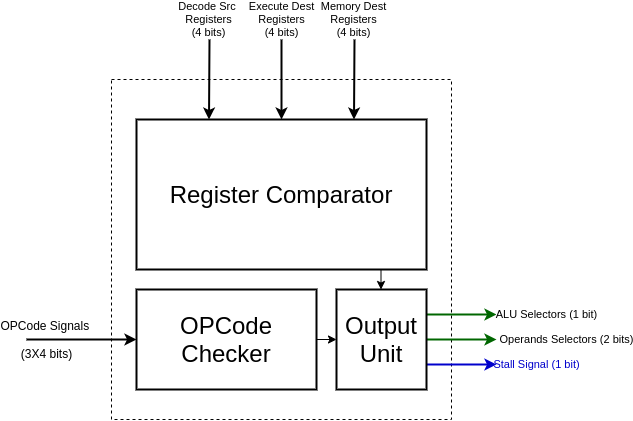
\includegraphics[width=0.8\textwidth]{images/hdu}
    \caption{Hazard Detection Unit Diagram}
    \label{fig:hdu}
\end{figure}

\subsection{Detection}

\subsubsection{Hazard Detection Unit (HDU)}

HDU consists of 3 parts:
\begin{itemize}
    \item \textbf{OPCode Checker:} checks the opcode of the current instruction to check whether it will cause data hazard or not. Also, it checks for \emph{load-use case}, in order to activate the stall signal.
    \item \textbf{Register Comparator:} compares the decode source registers with the destination registers of the execute and memory stages. Also, it compares the execute source registers with the destination registers of the memory stage.
    \item \textbf{Output Unit:} outputs stall signal in case of load and pop instructions (considering the branch special case). Also, it outputs ALU and decode operands selectors. 
\end{itemize}

\subsection{Handling}

\subsubsection{Stall}
Occurs only at Fetch and Decode stage, due to load(pop) use case.
\begin{itemize}
    \item Fetch same instruction (don't increment the program counter).
    \item Latch IF/ID buffer with the same values.
    \item Freeze Decode stage.
    \item Clear ID/EX buffer.
\end{itemize}

\subsubsection{Data Forwarding}
\begin{itemize}
    \item EX/MEM buffer $->$ Execute / Decode.
    \item ID/EX buffer $->$ Decode.
\end{itemize}

\section{Control Hazards}

\subsection{Detection}
The branch address calculation occurs in the Decode stage. So, the hazard might affect only the Fetch stage, which will be flushed in case of wrong address prediction.

\subsection{Handling}
\begin{itemize}
    \item At Fetch stage, always check the branch predictor and calculate the next address accordingly.
    \item At Decode stage, we have a \emph{Branch Address Unit} that checks whether the OPCode is of a branch operation. If so, it passes the address to the program counter and compares the correct address with the address of the counter to decide whether to flush the Fetch stage or not. 
\end{itemize}

\subsubsection{Flush}
Occurs only at Fetch Stage, due to wrong branch prediction at Decode stage.
\begin{itemize}
    \item Load new address in the program counter.
    \item Remove fetched instructions from IF/ID buffer.
\end{itemize}

\subsubsection{Dynamic Branch Prediction}
We use 2-bit branch predictor, which is a hash table of \emph{Finite State Machines} (FSMs) to predict whether the branch will be taken (1) or not (0) at each individual branch address.

\section{Software Solutions}
\label{sec:software}

There are some specialized software solutions done by the compiler. It can be summarized in:
\begin{itemize}
    \item Insertion of 1 NOP before each JZ operation to avoid data hazards in CCR.
    \item Insertion of 1 NOP before each STD and PUSH operation to avoid data hazards due to delay in data memory.
    \item Insertion of 4 NOPs after each RTI or RET operation to avoid unnecessary instruction fetch.
    \item Insertion of 4 NOPs before each CALL or JMP operation to have enough time for all results to be written back to register file, as JMP and CALL don't activate branch address check in decode stage.
\end{itemize}

\part{Memory Cache Design}
\subsection{Intuition and Assumptions}
\label{intuitionSection}
    Since data bus is $16-bits$ in width ie. $word$; so the following sizes are in terms of $words$.
    
    Since we are dealing with ONE main memory that contains all the Data and Instructions,
    and two caches one for Data and the other is for Instructions.

    This Design proposes to divide the Main memory into two parts, one for Data and one for Instructions,
    the upper most part is saved for Data from \textit{address} $00000000000$ to $01111111111$, while the Instructions
    \textit{address} starts from $10000000000$ to $11111111111$.

    Considering this, the $LSB$ of the address will indicate whther that address is corresponding to
    an instruction ($1$) or data ($0$).

    These assumptions allow us to:
    \begin{itemize}
        \item Limit collisions (conflicts) since for each Cache the tag size is reduced
            to only two bits since the actual address is 10 bits.
        \item Create an internal pipeline between the instruction cache and data cache,
            since the instruction cache is used only for reading, and filled periodically, more on 
            that on section \nameref{workflowSection}.
        \item No dirty bit array is used for instruction cache.
    \end{itemize}
     
\subsection{Caches Size}
    What is Given:
    \begin{itemize}
        \item Main memory: $4KB = 2^{12}B =2^{11} W$
        \item Cache Size: $512 Bytes = 256Words$
        \item Block Size: $16B = 8W$
        \item Number of Rows/Slots: $32$
        \item Number of Caches: $2$ one for Data and one for Instructions.
    \end{itemize}

    Sizes:
    \begin{itemize}
        \item Each Cache is $256Words$
        \item Tags are 2 bits in width.
        \item Validity is only 1 bit.
        \item Dirty bit is used only in case of Data cache.
        \item Extra bits required in total: $32*(2+1) + 16*(1) = 112bits$
    \end{itemize}


\subsection{Workflow}
\label{workflowSection}
    \subsubsection{General Cache Design}
    As proposed in the \nameref{intuitionSection} section, two caches exist in the design.

    In order to increase efficiency; we propose this fig.\ref{fig:cacheDesign}:
    \begin{itemize}
        \item Initially the instruction cache is filled with the first $Block$.
        \item The propgram will start working as usually\dots
        \item If No memory instruction is produced, this means the Memory is Ideal..
        \item The Cache Controller requests more $Blocks$ of Instructions from main memory.
        \item Meanwhile if Data is required from memory to be read or written, it will wait 
            until the current block is retreived then the required $Data$ will be provided.
        \item Then the $Data$ request will be fullfilled.
        \item This means that Data Memory has higher priority unless the instruction cache is empty.
    \end{itemize}

    The following algorithm may make things more clear\dots

    \begin{algorithm}[H]
        \SetAlgoLined
        \While{True}{
            \uIf{Instruction Cache is Empty}{
                Fetch the Next Instruction.\;
            }
            \uElseIf{Memory is Free to be Used}{
                Fetch the Next Instruction.\;
            }
            \Else{
                \uIf{there is a Data Memory Instruction}{
                    \uIf{Memory is Busy}{
                        Queue it next\;
                    }\Else{
                        Operate Now\;
                    }
                }
            }
        }
        \caption{Cache Controller}
        \end{algorithm}
    
    \vspace{1cm}
    What makes this algorithm efficient is these two information, One: the Instruction cache
    can be written periodically, Two: the Rate of Memory Instruction is very low and the Number
    of memory instruction (such as $SW$ and $LD$) is less than other Instructions.

    \begin{figure}[H]
        \centering
        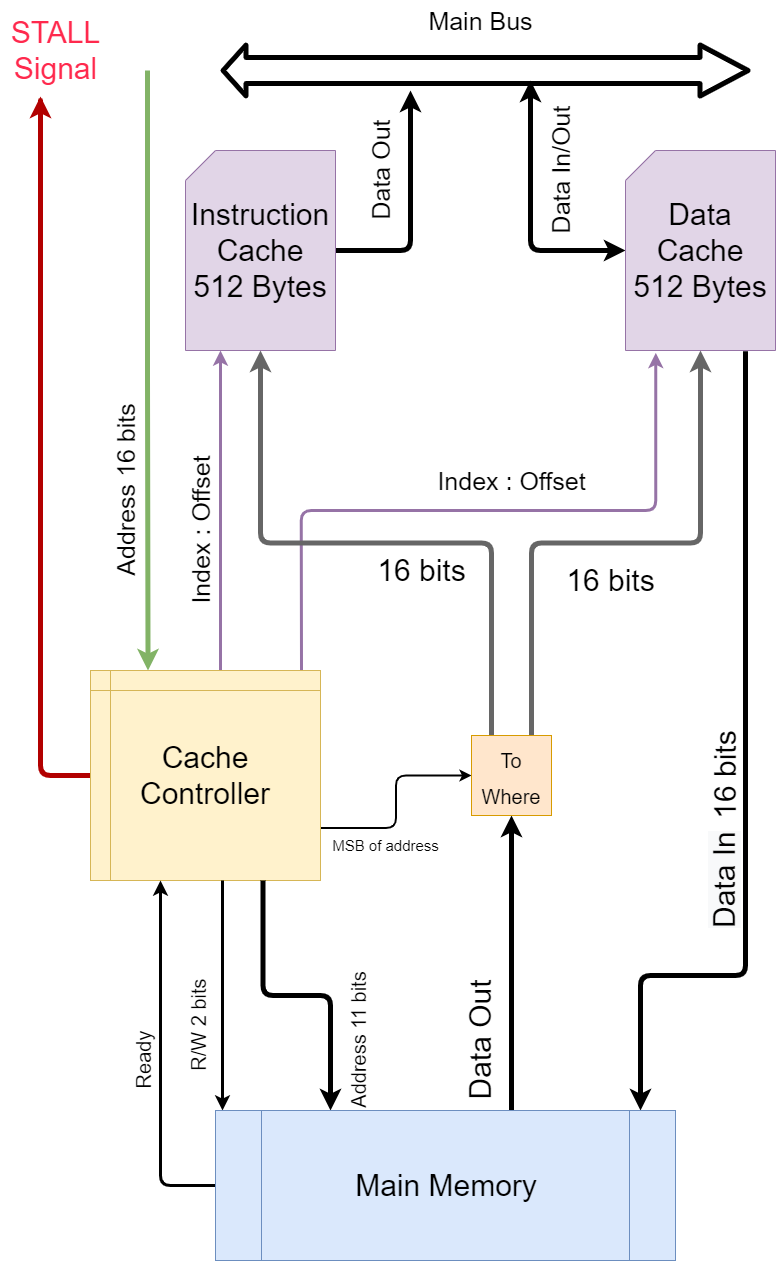
\includegraphics[width=\textwidth]{images/cache/full_cache_design.png}
        \caption{Cache Design}
        \label{fig:cacheDesign}
    \end{figure}

    \subsubsection{Data Cache Design}

    In the following flowchart fig.\ref{fig:dataCache} we illustrate how read and write operations are
    handled in our system.\newline

    Notes:
    \begin{itemize}
        \item These operations are related to $Data$ cache.
        \item When Valid bit equals 0, this means it's not valid, and vv.
        \item When Dirty bit equals 0. this means the block is not modified, and vv.
        \item $Circle A$ is responsible for reading from main memory.
        \item $Circle B$ is responsible for writing into main memory (Replacement).
        \item Replacement occurs only when read is demanded let's see why:
            \begin{itemize}
                \item when dirty bit is set, and that exact same block is needed for read or write operation
                \item If it's needed for read operation then the old block will be written first,
                    then the ordered block will be read, this is ordinary Replacement.
                \item and if it's needed for write operation, then if it's not valid or missed ordinary Replacement
                is requested,
                \item but if it was valid and tag is matched then we don't need to check the dirty bit
                \textbf{data can be overwritten without updating the main memory} and the dirty bit is set anyway.
            \end{itemize}
    \end{itemize}


    \begin{figure}[H]
        \centering
        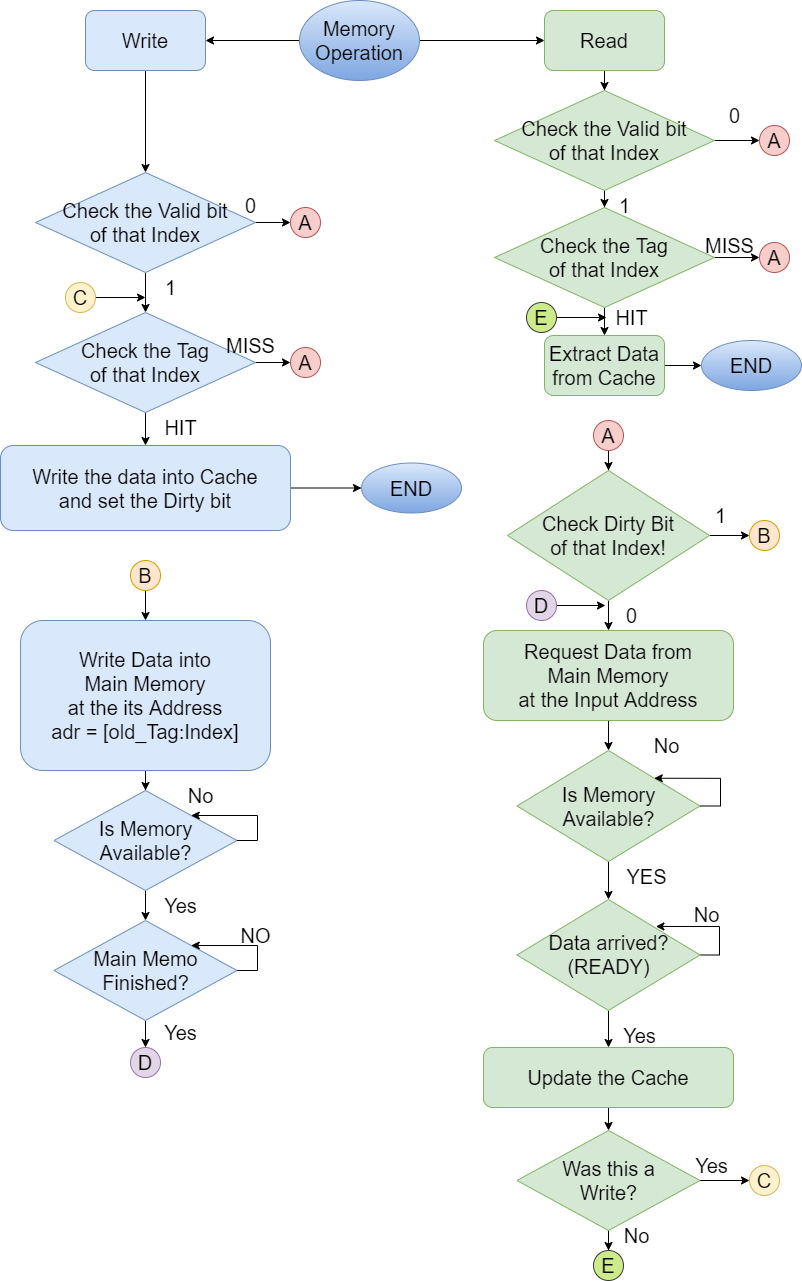
\includegraphics[width=\textwidth]{images/cache/cache_system_flowchart.png}
        \caption{Data Cache R/W}
        \label{fig:dataCache}
    \end{figure}



\part{Implementation Overview}
\section{Completeness}
The processor is completely implemented except for \textbf{memory cache system}, which is already designed. However, we ran out of time trying to integrate it to our current implementation.

So, we reverted back to the two memories, \emph{Harvard} architecture. However, we included the cache system design in this report to share our thinking.

\section{Functionality}
The implemented processor, with \emph{Harvard} architecture, completely works with correct functionalities and hazard handling.

However, we still have the following issues:
\begin{itemize}
    \item Some instructions cause data hazards, that can't be completely solved by HDU. So, we had to use some software solutions to handle it, due to time constraints (Refer to \ref{sec:software}).
\end{itemize}

\section{General Notes}
\begin{itemize}
    \item Fetch stage outputs a single \emph{NOP} instruction, in case of \emph{Interrupt}, \emph{CALL}, \emph{JZ} and \emph{JMP}, due to the delay of reading data (PC values or branch address) from register file.
    \item Flushing happens only to the fetch stage, in case of incorrect predicted branch address for \emph{JZ} instruction.
    \item The compiler should add an extra instruction \emph{END} to the end of the assembly program to mark the end of the code and terminate the simulator.
    \item We used \emph{ghdl} as a \emph{VHDL} compiler and \emph{GTKWave} as a simulator throughout the development process for fast development and debugging. We included our development setup, along with the main deliverables of the project. 
\end{itemize}

\part{Implementation Analysis}
\section{Provided Test Cases}
In this section, we provide the output wave for the provided test cases. We show both full code results and the results of disabled hazard handling. Also, we show the wave of handling hazards through NOPs.

\subsection{One Operand Test Case}

\subsubsection{Full Code}
The figures \ref{fig:1op_reg_1} and \ref{fig:1op_reg_2} show the output wave of full code.
\begin{figure}[H]
    \centering
    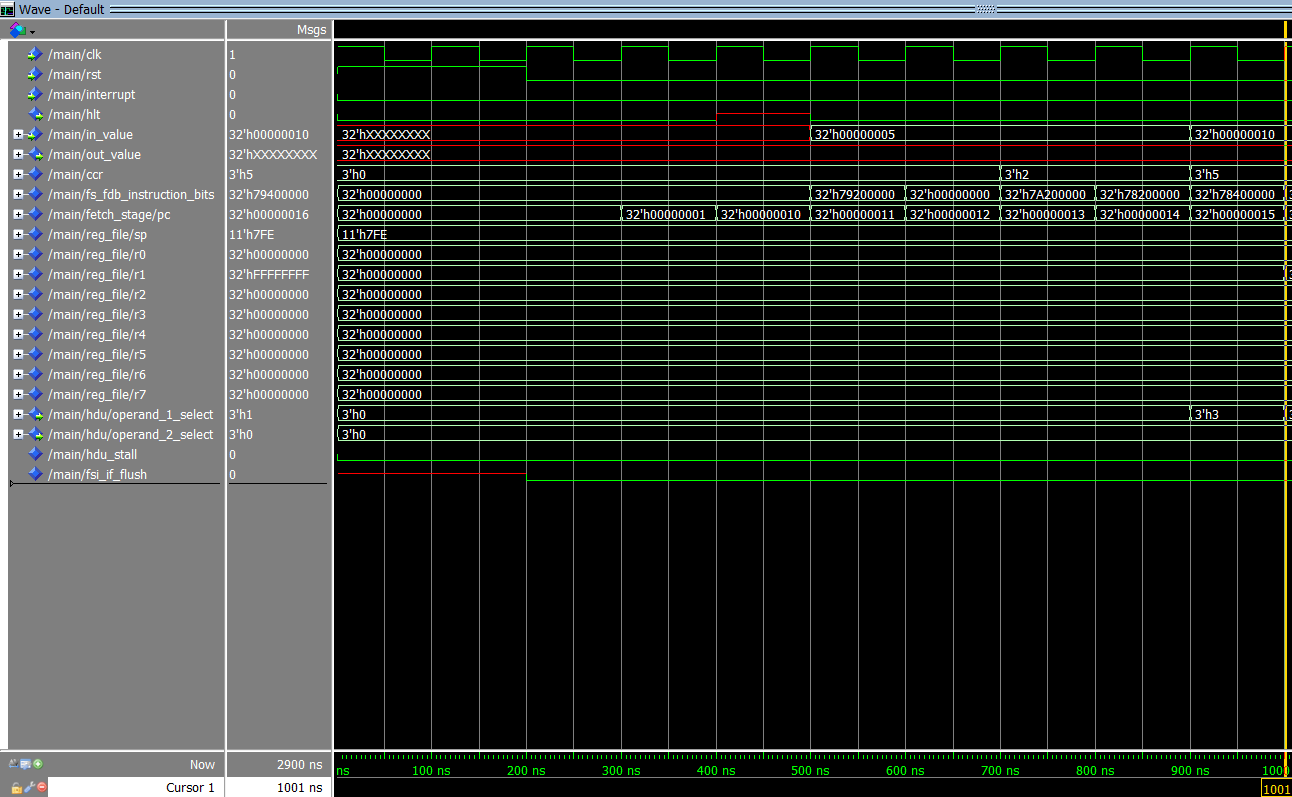
\includegraphics[width=0.9\textwidth]{images/test_cases/one_operand/OneOperand_regular_1.PNG}
    \caption{One Operand Full Code Output wave 1}
    \label{fig:1op_reg_1}
\end{figure}

\begin{figure}[H]
    \centering
    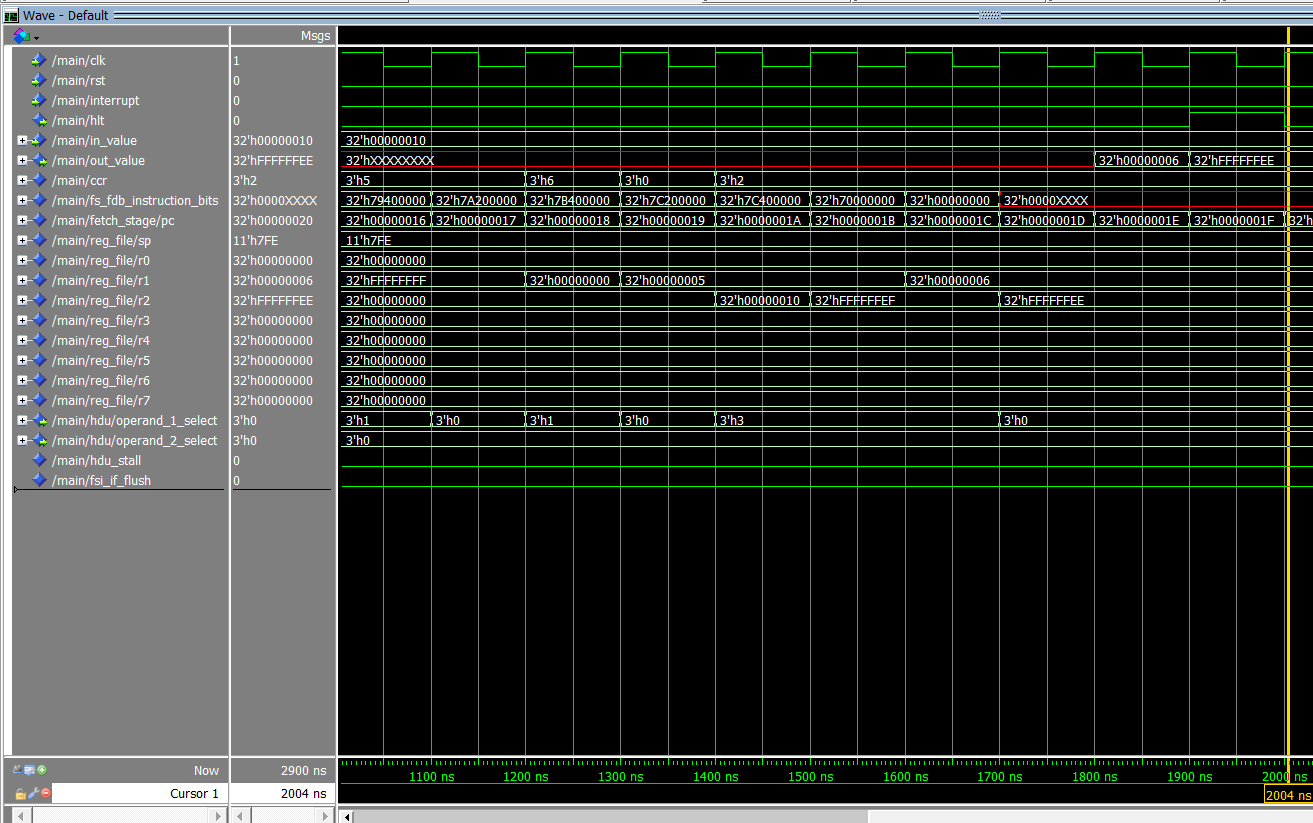
\includegraphics[width=0.9\textwidth]{images/test_cases/one_operand/OneOperand_regular_2.PNG}
    \caption{One Operand Full Code Output wave 2}
    \label{fig:1op_reg_2}
\end{figure}

\subsubsection{No Forwarding}
The figures \ref{fig:1op_no_1} and \ref{fig:1op_no_2} show the output wave of code with no forwarding.
\begin{figure}[H]
    \centering
    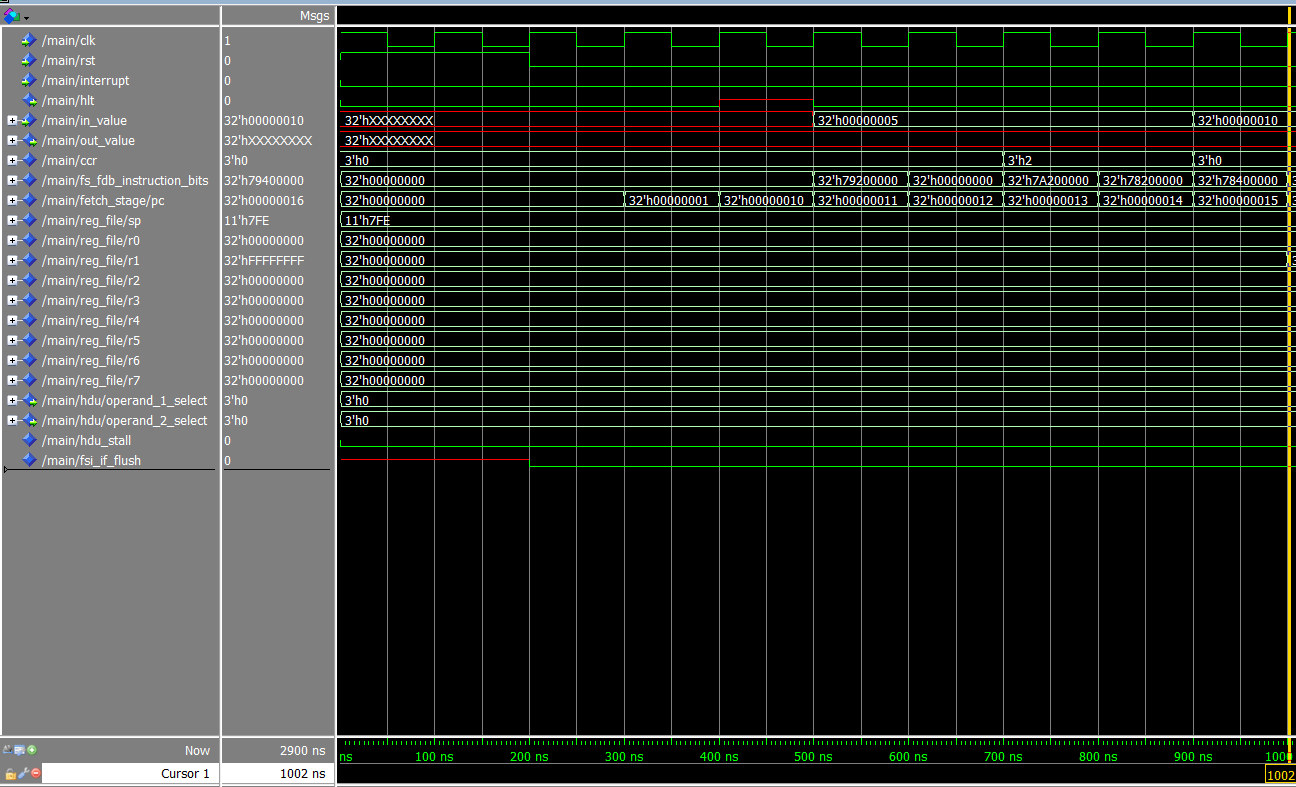
\includegraphics[width=0.9\textwidth]{images/test_cases/one_operand/OneOperand_no_forward_1.PNG}
    \caption{One Operand No Forwarding Output wave 1}
    \label{fig:1op_no_1}
\end{figure}

\begin{figure}[H]
    \centering
    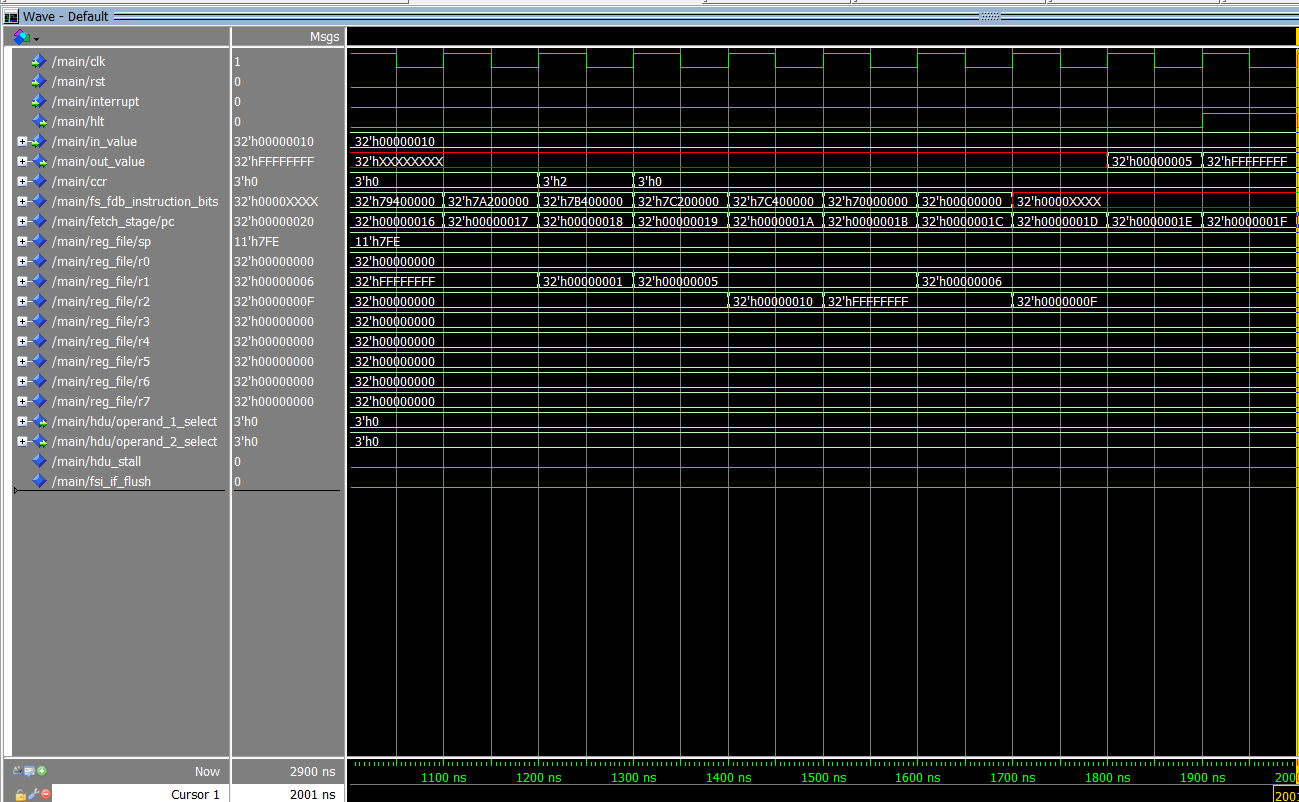
\includegraphics[width=0.9\textwidth]{images/test_cases/one_operand/OneOperand_no_forward_2.PNG}
    \caption{One Operand No Forwarding Output wave 2}
    \label{fig:1op_no_2}
\end{figure}

\subsubsection{NOPs Solution}
The figures \ref{fig:1op_nop_1}, \ref{fig:1op_nop_2} and \ref{fig:1op_nop_3} show the output wave of code with NOPs solution.
\begin{figure}[H]
    \centering
    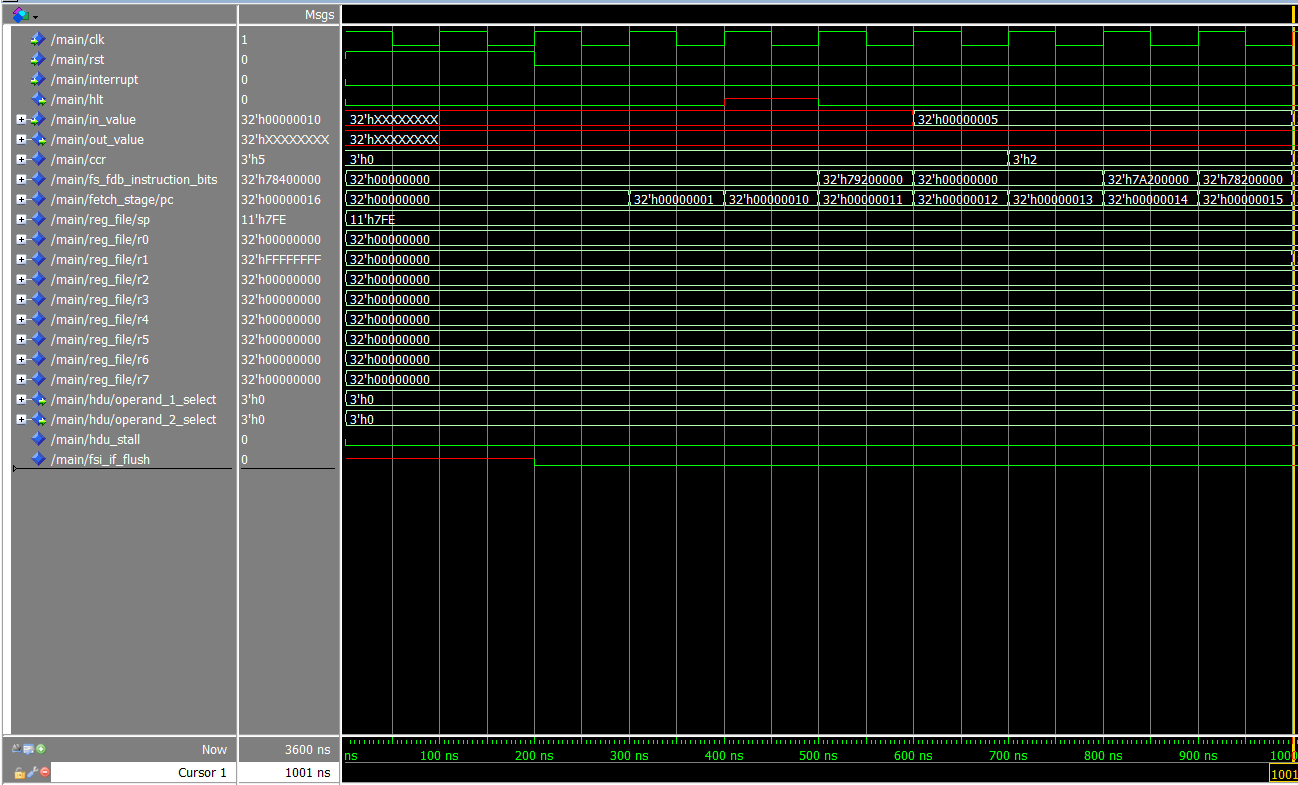
\includegraphics[width=0.9\textwidth]{images/test_cases/one_operand/OneOperand_NOP_1.PNG}
    \caption{One Operand NOPs Solution Output wave 1}
    \label{fig:1op_nop_1}
\end{figure}

\begin{figure}[H]
    \centering
    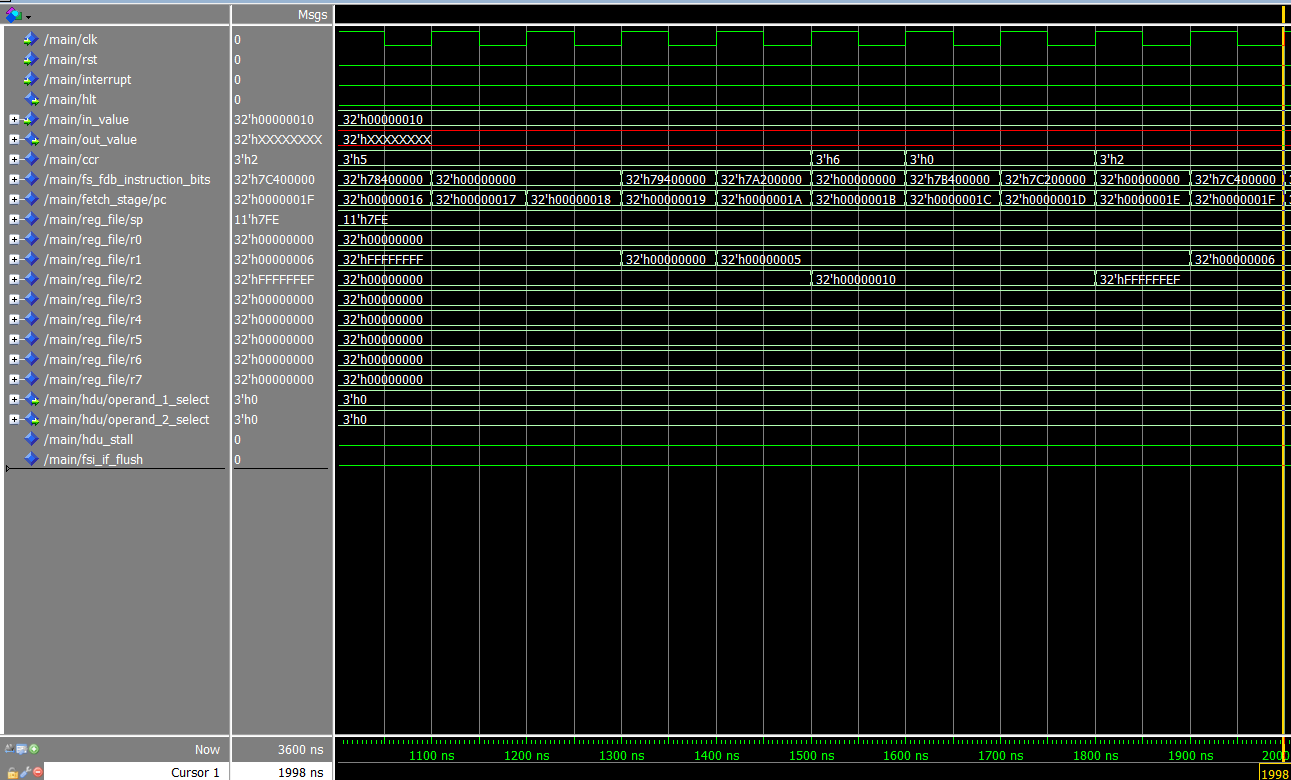
\includegraphics[width=0.9\textwidth]{images/test_cases/one_operand/OneOperand_NOP_2.PNG}
    \caption{One Operand NOPs Solution Output wave 2}
    \label{fig:1op_nop_2}
\end{figure}

\begin{figure}[H]
    \centering
    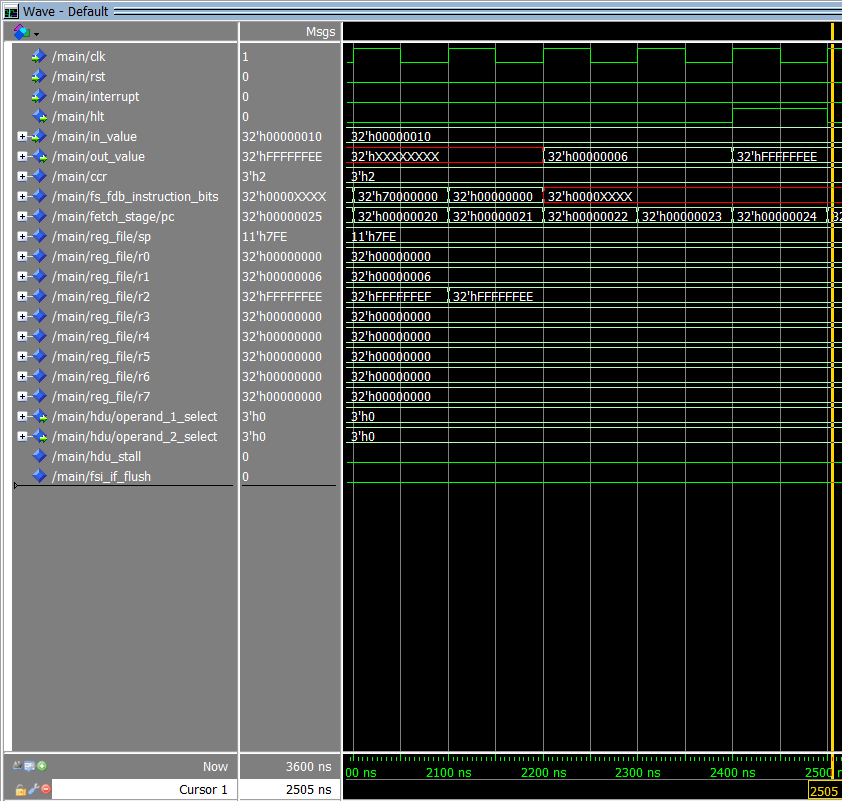
\includegraphics[width=0.9\textwidth]{images/test_cases/one_operand/OneOperand_NOP_3.PNG}
    \caption{One Operand NOPs Solution Output wave 3}
    \label{fig:1op_nop_3}
\end{figure}


\subsection{Two Operand Test Case}

\subsubsection{Full Code}
The figures \ref{fig:2op_reg_1}, \ref{fig:2op_reg_2} and \ref{fig:2op_reg_3} show the output wave of full code.
\begin{figure}[H]
    \centering
    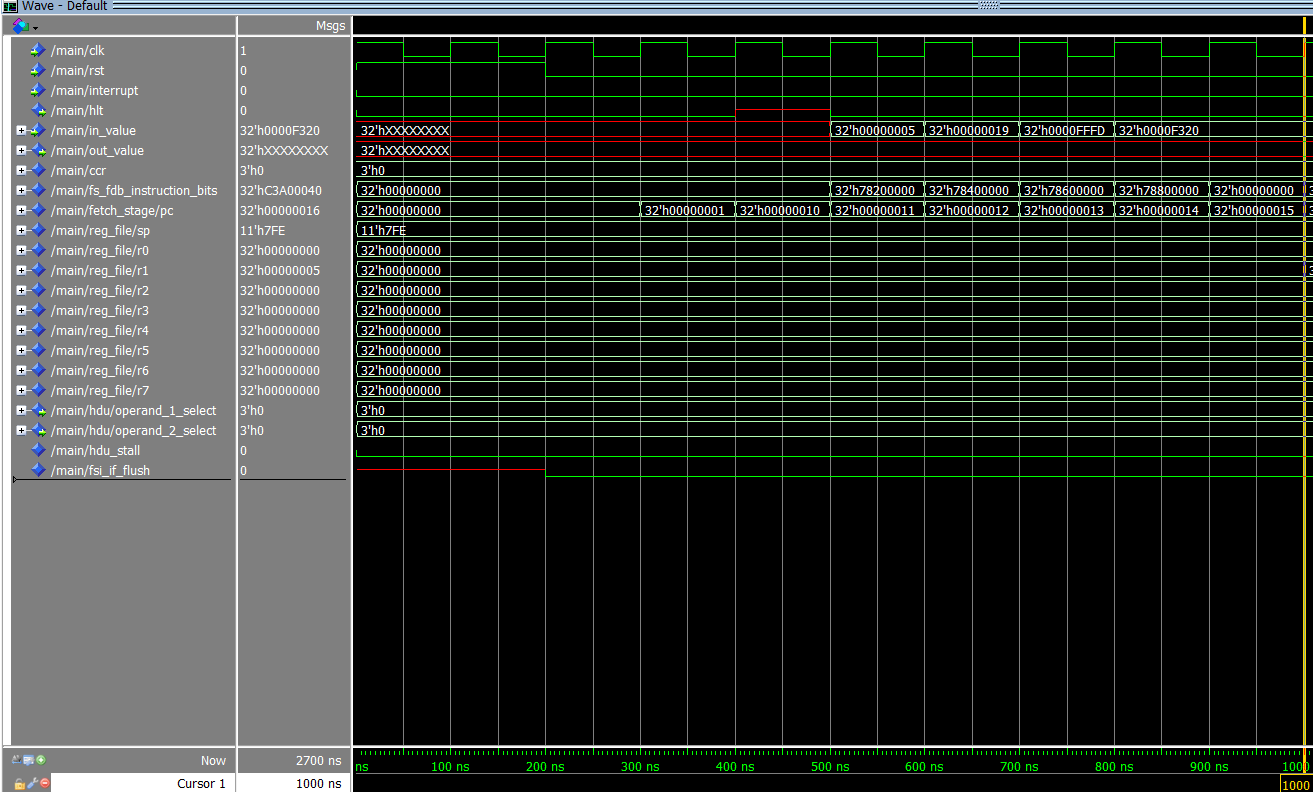
\includegraphics[width=0.9\textwidth]{images/test_cases/two_operand/TwoOperand_regular_1.PNG}
    \caption{Two Operand Full Code Output wave 1}
    \label{fig:2op_reg_1}
\end{figure}

\begin{figure}[H]
    \centering
    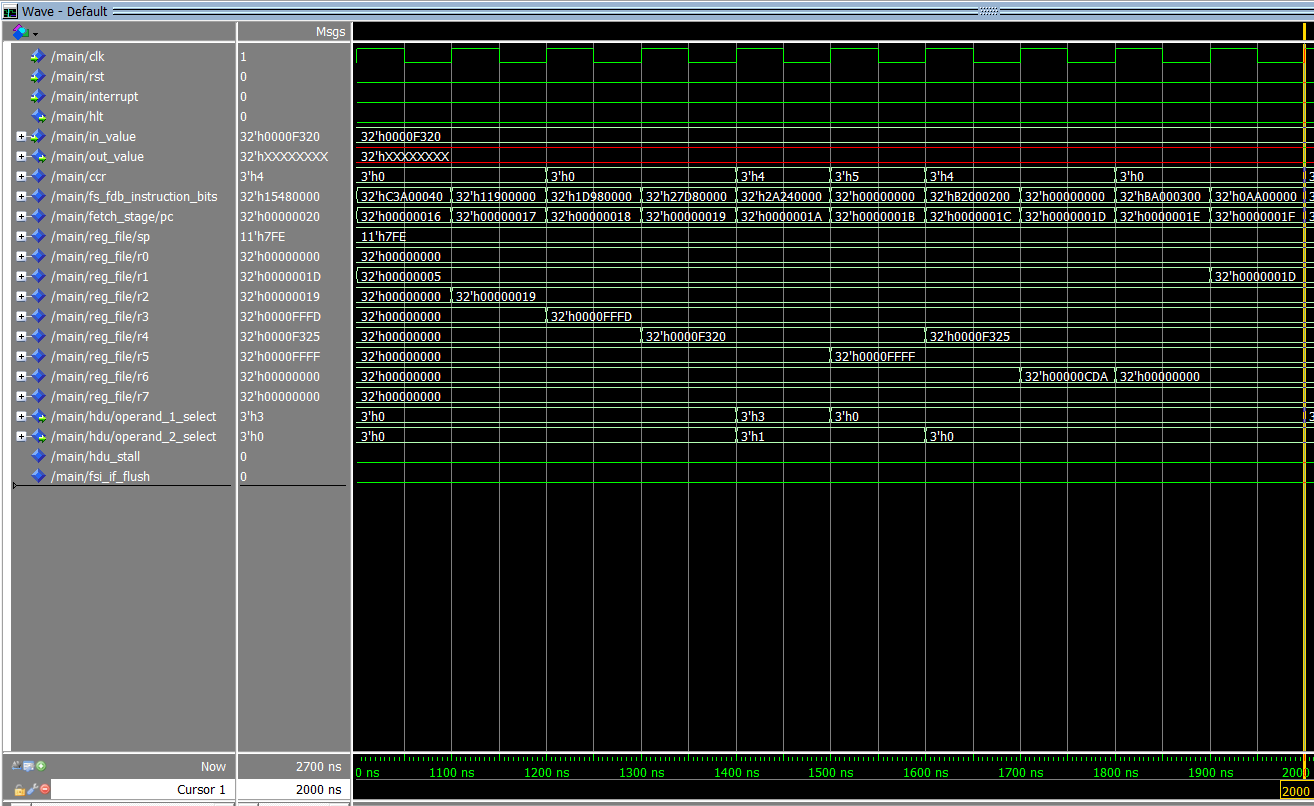
\includegraphics[width=0.9\textwidth]{images/test_cases/two_operand/TwoOperand_regular_2.PNG}
    \caption{Two Operand Full Code Output wave 2}
    \label{fig:2op_reg_2}
\end{figure}

\begin{figure}[H]
    \centering
    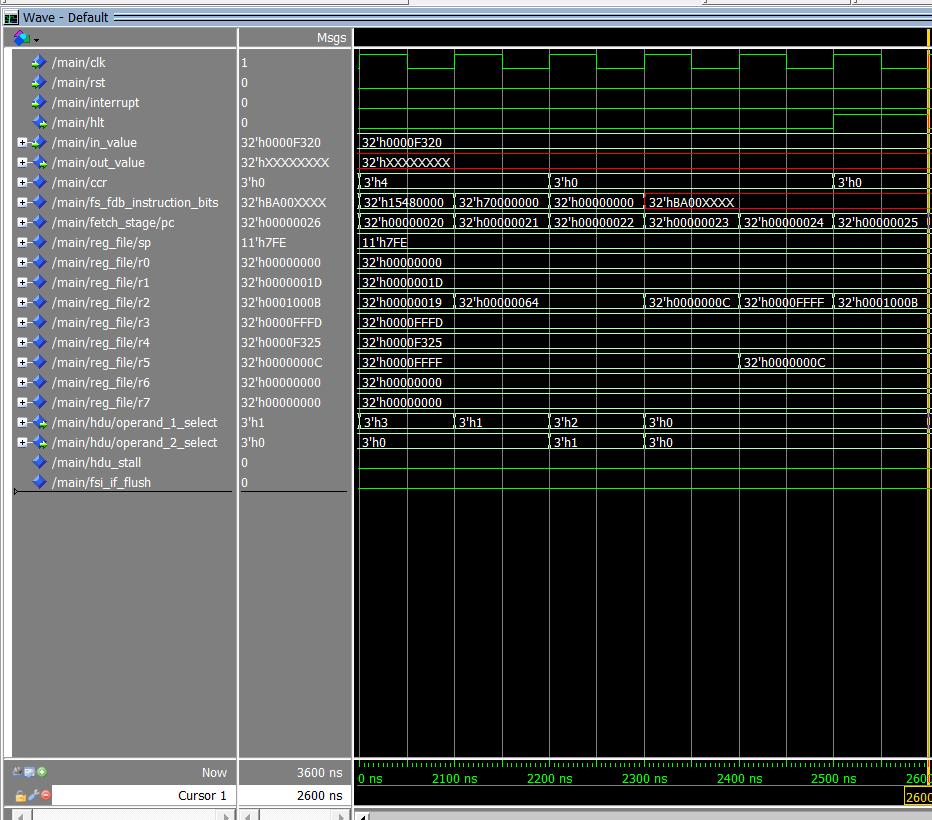
\includegraphics[width=0.9\textwidth]{images/test_cases/two_operand/TwoOperand_regular_3.PNG}
    \caption{Two Operand Full Code Output wave 3}
    \label{fig:2op_reg_3}
\end{figure}

\subsubsection{No Forwarding}
The figures \ref{fig:2op_no_1}, \ref{fig:2op_no_2} and \ref{fig:2op_no_3} show the output wave of code with no forwarding.
\begin{figure}[H]
    \centering
    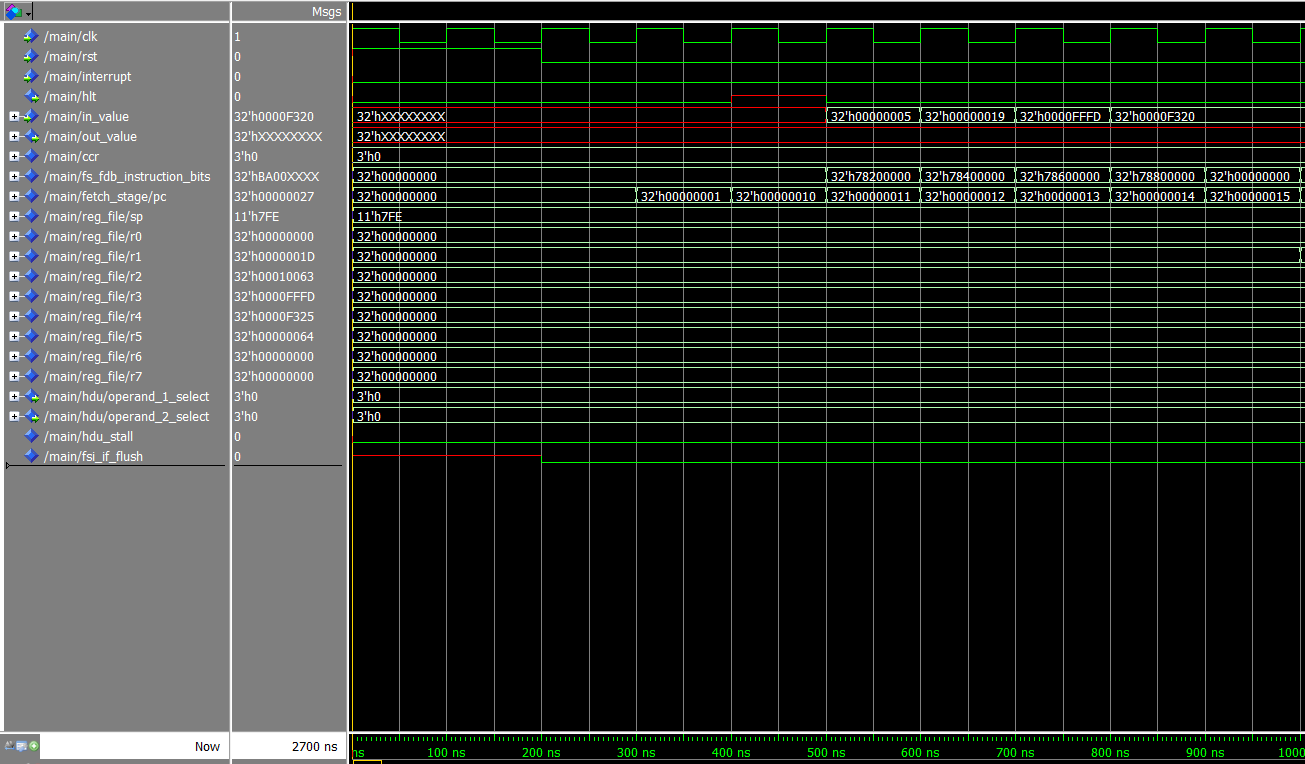
\includegraphics[width=0.9\textwidth]{images/test_cases/two_operand/TwoOperand_no_forward_1.PNG}
    \caption{Two Operand No Forwarding Output wave 1}
    \label{fig:2op_no_1}
\end{figure}

\begin{figure}[H]
    \centering
    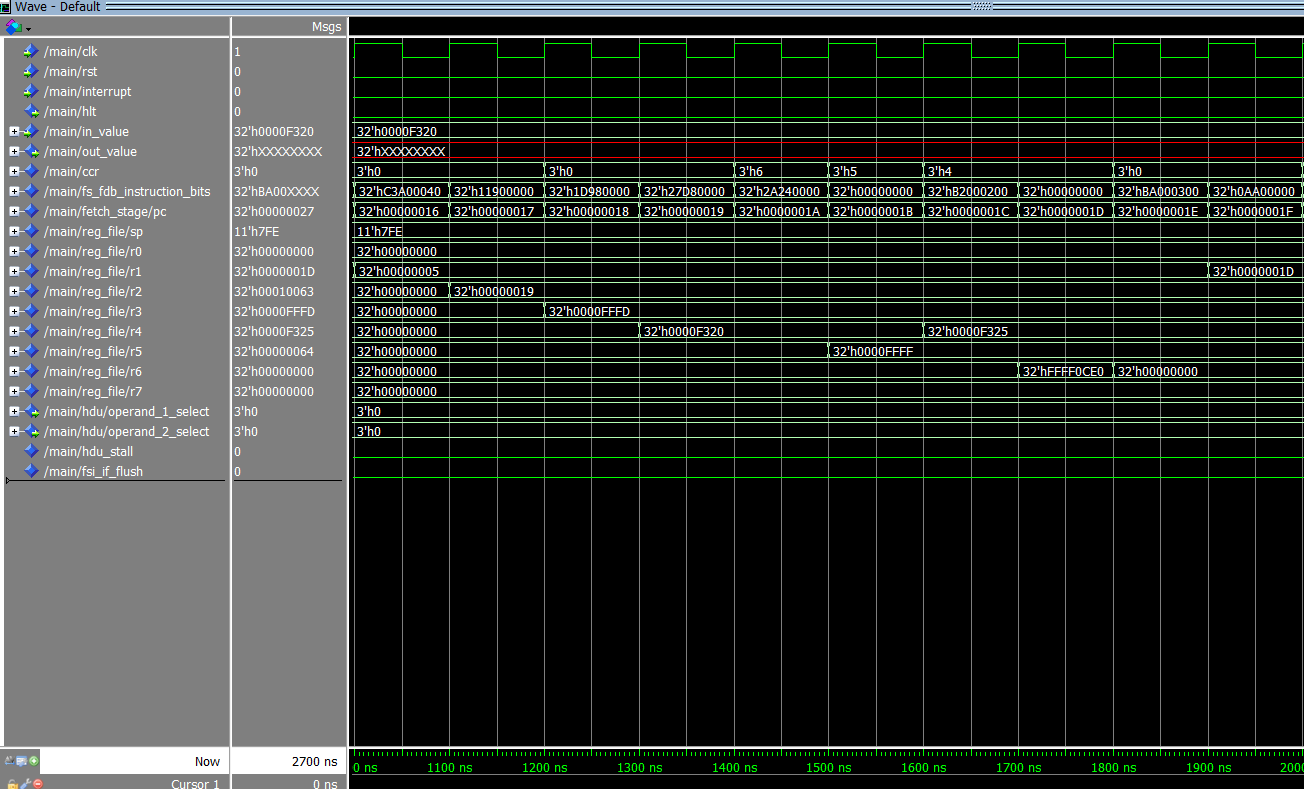
\includegraphics[width=0.9\textwidth]{images/test_cases/two_operand/TwoOperand_no_forward_2.PNG}
    \caption{Two Operand No Forwarding Output wave 2}
    \label{fig:2op_no_2}
\end{figure}

\begin{figure}[H]
    \centering
    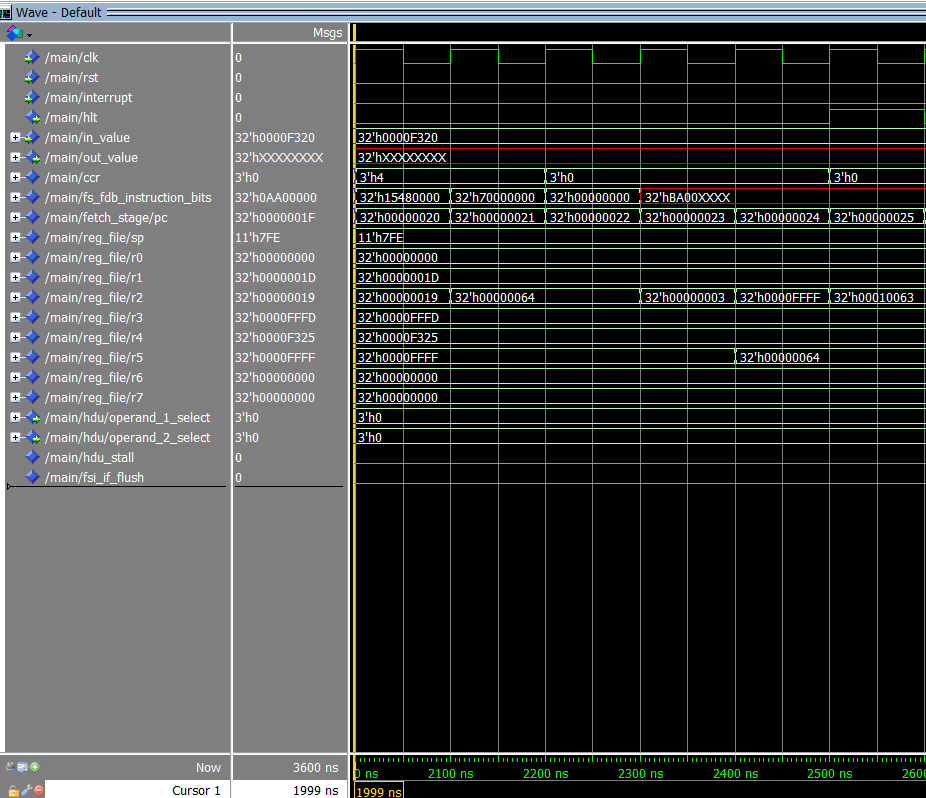
\includegraphics[width=0.9\textwidth]{images/test_cases/two_operand/TwoOperand_no_forward_3.PNG}
    \caption{Two Operand No Forwarding Output wave 3}
    \label{fig:2op_no_3}
\end{figure}

\subsubsection{NOPs Solution}
The figures \ref{fig:2op_nop_1}, \ref{fig:2op_nop_2}, \ref{fig:2op_nop_3} and \ref{fig:2op_nop_4} show the output wave of code with NOPs solution.
\begin{figure}[H]
    \centering
    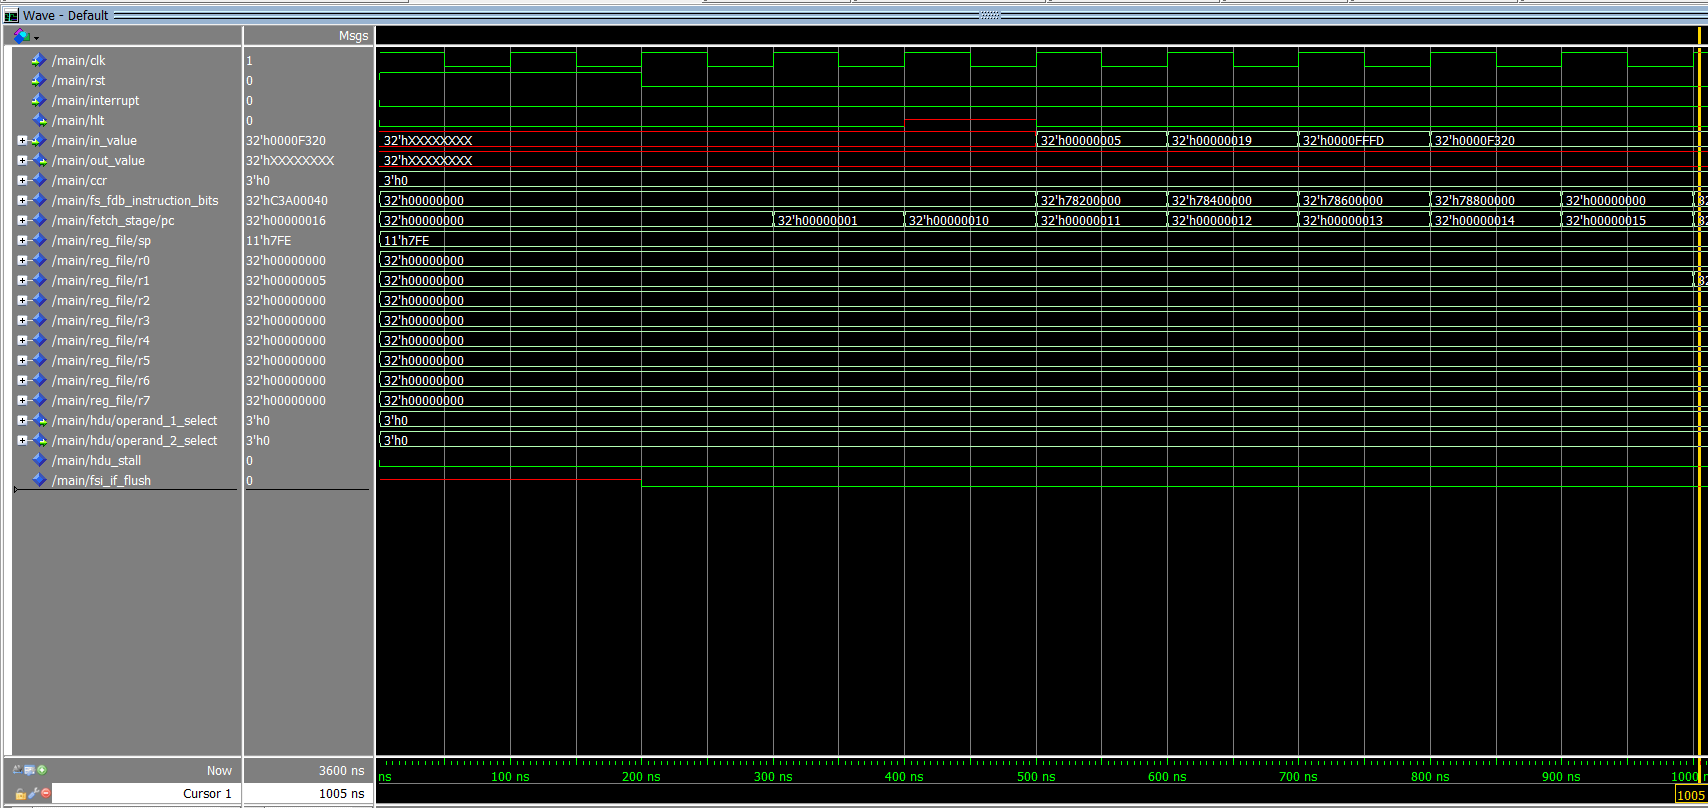
\includegraphics[width=0.9\textwidth]{images/test_cases/two_operand/TwoOperand_NOP_1.PNG}
    \caption{Two Operand NOPs Solution Output wave 1}
    \label{fig:2op_nop_1}
\end{figure}

\begin{figure}[H]
    \centering
    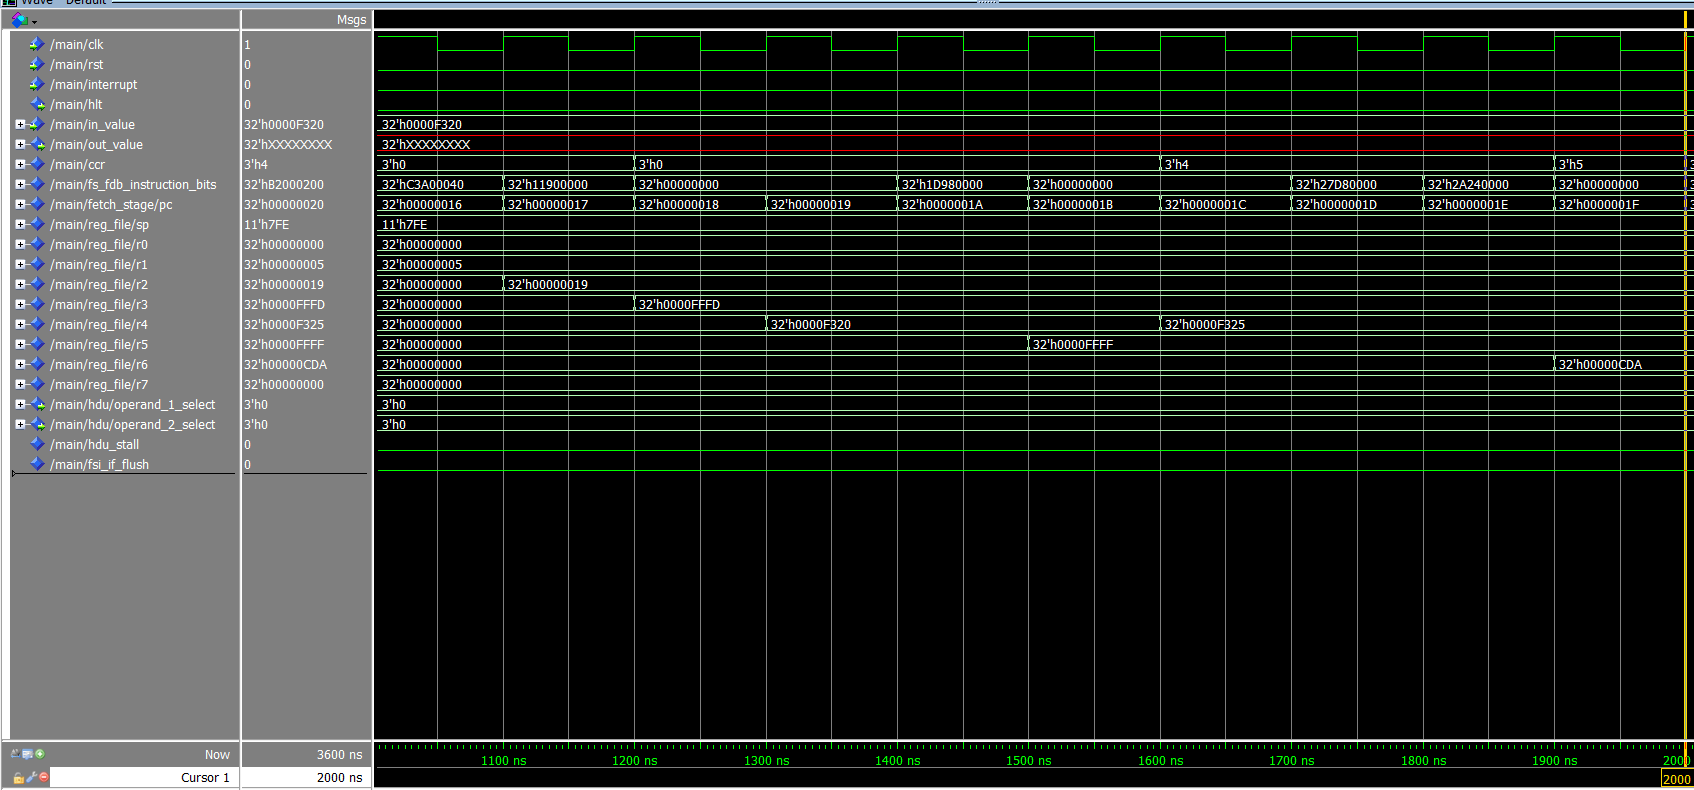
\includegraphics[width=0.9\textwidth]{images/test_cases/two_operand/TwoOperand_NOP_2.PNG}
    \caption{Two Operand NOPs Solution Output wave 2}
    \label{fig:2op_nop_2}
\end{figure}

\begin{figure}[H]
    \centering
    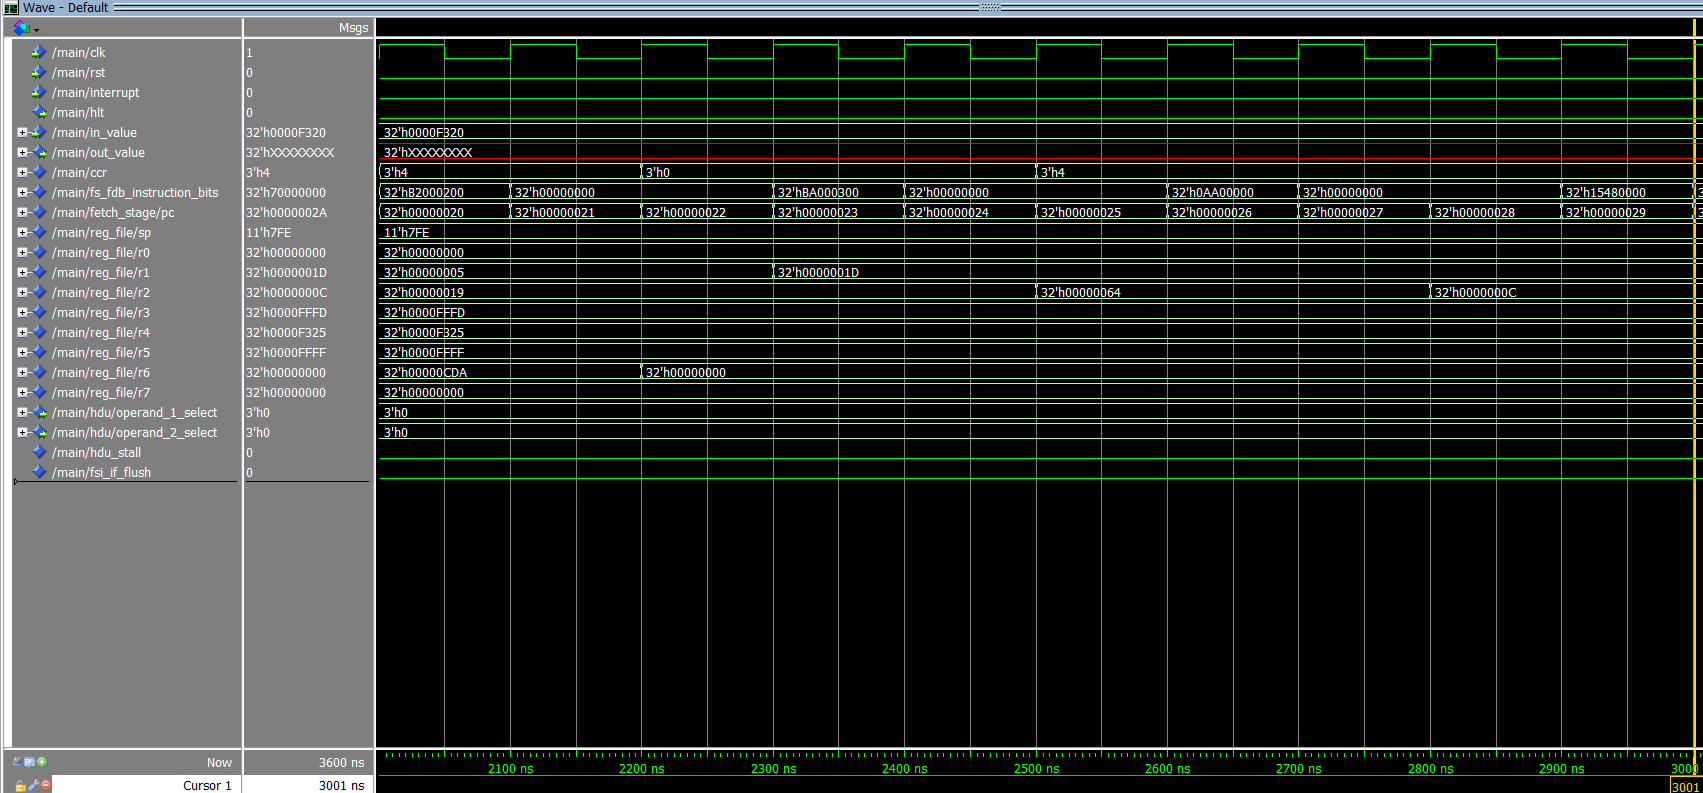
\includegraphics[width=0.9\textwidth]{images/test_cases/two_operand/TwoOperand_NOP_3.PNG}
    \caption{Two Operand NOPs Solution Output wave 3}
    \label{fig:2op_nop_3}
\end{figure}

\begin{figure}[H]
    \centering
    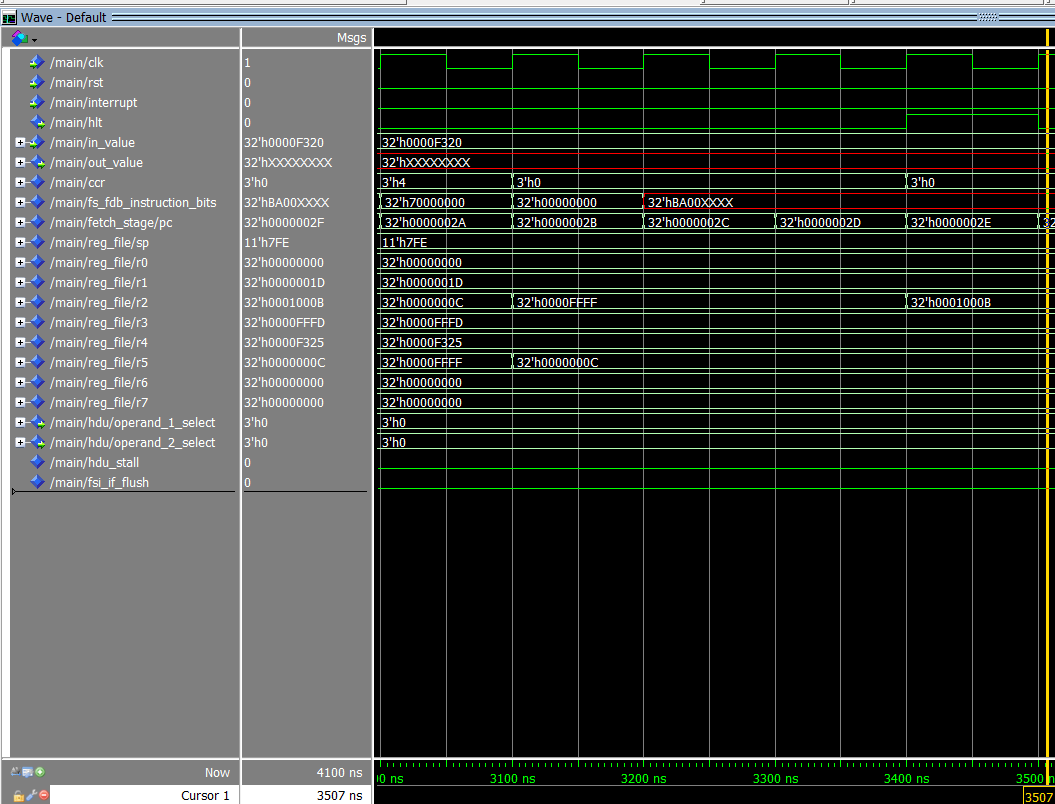
\includegraphics[width=0.9\textwidth]{images/test_cases/two_operand/TwoOperand_NOP_4.PNG}
    \caption{Two Operand NOPs Solution Output wave 4}
    \label{fig:2op_nop_4}
\end{figure}

\subsection{Memory Test Case}

\subsection{Branch Test Case}

\subsection{Branch Prediction Test Case}

\subsection{Memory Cache Test Case}
Memory cache system is not implemented. 

\section{Complete Hazard Analysis}

\end{document}
